\documentclass[11pt]{amsart}
\usepackage[T1]{fontenc}
\usepackage[utf8]{inputenc}
\usepackage{lmodern}
\usepackage{amsmath,amssymb,amsthm,mathtools}
\usepackage[margin=1in]{geometry}
\usepackage{microtype,enumitem,booktabs,array,graphicx,xcolor}
\usepackage{needspace}
\usepackage{tikz}
\usetikzlibrary{arrows.meta,calc,patterns,positioning}
\usepackage[hypertexnames=false,colorlinks=true,linkcolor=blue!45!black,citecolor=blue!45!black,urlcolor=blue!45!black]{hyperref}
\usepackage[capitalise,nameinlink,noabbrev]{cleveref}
\hypersetup{pdftitle={No bigeodesics in planar first-passage percolation},pdfauthor={OpenAI}}
\newtheorem{theorem}{Theorem}[section]
\newtheorem{proposition}[theorem]{Proposition}
\newtheorem{lemma}[theorem]{Lemma}
\newtheorem{corollary}[theorem]{Corollary}
\theoremstyle{definition}
\newtheorem{definition}[theorem]{Definition}
\theoremstyle{remark}
\newtheorem{remark}[theorem]{Remark}
\newcommand{\Z}{\mathbb Z}
\newcommand{\R}{\mathbb R}
\newcommand{\PP}{\mathbb P}
\newcommand{\EE}{\mathbb E}
\newcommand{\eps}{\varepsilon}
\DeclareMathOperator{\Dir}{Dir}
\DeclareMathOperator{\TV}{TV}
\DeclareMathOperator{\Var}{Var}
\allowdisplaybreaks[2]
\raggedbottom
\setlength{\emergencystretch}{1em}
\setlist{itemsep=3pt,topsep=5pt}
\title{No bigeodesics in planar first-passage percolation}
\author{OpenAI}
\date{September 24, 2026}
\begin{document}
\begin{abstract}
We prove that planar first-passage percolation with independent identically
distributed nonnegative nonatomic edge weights has almost surely no doubly infinite
geodesic, provided the minimum of four independent weights has finite second
moment. This resolves the planar no-bigeodesics conjecture under that moment
assumption. The conclusion rules out all bigeodesics simultaneously, without
any regularity assumption on the limit shape.
\end{abstract}
\maketitle
\section{Introduction}
\label{sec:introduction}

First-passage percolation, introduced by Hammersley and
Welsh~\cite{HammersleyWelsh1965}, equips a lattice with a random metric
by assigning independent passage times to its edges. A basic question asks
whether this metric can contain a doubly infinite minimizing path.
Such a path, called a \emph{bigeodesic}, is a random analogue of a
complete minimizing geodesic in a noncompact metric space.
The question was attributed to Furstenberg by
Kesten~\cite[Remark 9.22]{Kesten}.
The planar no-bigeodesics conjecture asserts that bigeodesics are absent
for iid continuous edge-weight laws; see
\cite[Conjecture 1 and the discussion preceding it]{DamronHanson}.
We prove the conjecture under the minimum-of-four second-moment
assumption.

Let \(\mathcal E\) denote the unoriented nearest-neighbor edges of
\(\Z^2\). Give these edges independent weights \(t_e\) with common
Borel probability law \(G\) on \([0,\infty)\). For vertices \(x,y\),
let \(T(x,y)\) be the infimum of the costs of finite nearest-neighbor
walks from \(x\) to \(y\), with each edge traversal charged its weight.

\begin{theorem}\label{thm:main}
Suppose that \(G\) has no atoms and that, for independent
\(X_1,X_2,X_3,X_4\) with law \(G\),
\begin{equation}\label{eq:minimum-moment}
 \EE\!\left[\min\{X_1,X_2,X_3,X_4\}^{\,2}\right]<\infty.
\end{equation}
Then, with probability one, there is no sequence
\((v_i)_{i\in\Z}\) of pairwise distinct vertices with consecutive
vertices adjacent and
\[
 \sum_{k=i}^{j-1}t_{\{v_k,v_{k+1}\}}=T(v_i,v_j)
 \qquad\text{for every }i<j.
\]
\end{theorem}

The conclusion excludes all bigeodesics in one probability-one event.
In particular, an end direction may depend on the environment.
The law \(G\) may be singular continuous or have bounded support,
and \(\EE t_e\) may be infinite. We assume no differentiability,
strict convexity, or curvature of the limit shape.
Theorem~\ref{thm:main} resolves the planar no-bigeodesics conjecture
positively in the class \eqref{eq:minimum-moment}; it does not
assert the moment-free formulation.

\subsection*{Background}
The study of infinite geodesics and Busemann functions developed through
work of Newman~\cite{Newman1995}, Hoffman~\cite{Hoffman2005,Hoffman2008},
and the stationary constructions of Damron and
Hanson~\cite{DamronHanson2014}. Directional results connect geodesics
to the geometry of the limit shape. Licea and Newman proved coalescence
for each direction in a deterministic set of full Lebesgue measure and
excluded bigeodesics whose two end-directions are prescribed in that
set~\cite{LiceaNewman}; see also
\cite[Theorem~3.1 and Remark~2 after Theorem~1]{DamronHanson}.
This coalescence result requires no curvature assumption.
The complementary assertion that every ray has a direction and that
rays exist in every direction was established by Newman under an
exponential moment and uniform curvature
\cite[Theorem~2.1]{Newman1995}. Damron and Hanson subsequently obtained
one-end exclusions in fixed tangent-contact sectors under local
differentiability assumptions~\cite[Theorem~1]{DamronHanson}.
Their full iid hypothesis A1$'$ already allows
\eqref{eq:minimum-moment}; the distinction here is the absence of shape
assumptions and the simultaneous treatment of every possible path.

Wehr and Woo excluded bigeodesics in the half-plane restricted metric
under a finite individual-edge mean~\cite{WehrWoo1998}.
Auffinger, Damron, and Hanson removed that moment assumption for
continuous iid weights~\cite[Appendix~C]{AuffingerDamronHanson2015}
and proved coalescence and finite backward clusters for the associated
boundary-limit geodesic forest
\cite[Theorem~1.5]{AuffingerDamronHanson2015}.
Brito, Damron, and Hanson proved the absence of doubly infinite directed
paths in geodesic graphs obtained as limits of point-to-hyperplane
constructions in a fixed direction~\cite{BritoDamronHanson2023}.
Their iid hypothesis also gives \eqref{eq:minimum-moment} in two
dimensions, but their selected graphs need not contain every geodesic
of the metric. Alexander proved simultaneous absence of bigeodesics
under additional exponential-moment, uniform-curvature, and quantitative
fluctuation assumptions~\cite{Alexander2023}.

Ahlberg and Hoffman developed a structural theory of random
coalescing geodesics that assigns an asymptotically linear Busemann
function to every ray, without imposing shape regularity
\cite{AhlbergHoffman}.
Their results also give uniqueness, coalescence, and backward
finiteness for each fixed functional in a deterministic closed set.
These conclusions, stated in \Cref{thm:structure}, are the structural
inputs to our proof. We use them with the boundary comparison in
Appendix~\ref{sec:boundary-comparison}, which replaces a boundary-expectation
step without requiring integrability of restricted passage times.
Related developments include sublinear growth of planar geodesic
trees~\cite{AhlbergHansonHoffman} and quantitative coalescence and
midpoint estimates under stronger distributional and geometric
hypotheses~\cite{DembinElboimPeled}.

There is a quantifier issue that those inputs alone do not settle:
almost-sure uniqueness for each fixed functional does not imply
simultaneous uniqueness at every environment-dependent functional.
A bigeodesic, if one existed, could select such an exceptional
functional. Our argument treats these random functionals directly
and then uses an increasing passage-time cost to exclude all
remaining candidates.

\subsection*{The argument}
A ray \(p\) has a Busemann function
\[
 B_p(x,y)=\lim_{j\to\infty}
          \bigl(T(x,p_j)-T(y,p_j)\bigr)
\]
with a linear asymptote \(\rho_p\), which we call its label.
The labels of the two ends of a bigeodesic are opposite.
After a countable reduction, it suffices to exclude bigeodesics whose
upper labels lie in one compact sector of the dual unit circle.
The horizontal coordinate \(r(\rho)=\rho(e_1)\) orders this sector;
write \(W\) for its width in that coordinate.

The contradiction is a finite budget for passage-time increases.
On a horizontal grid of spacing \(l\), we mark sites by selecting
bigeodesics in finitely increased environments. A marked path acquires
an extra cost of at least \(M\) on an initial portion.
Partition the label sector into bins with deterministic endpoints.
The selected arms and the base rays used for comparison are required
to satisfy common deterministic cone bounds.
When the marks in each bin are sufficiently separated, comparison
with rays at those endpoints charges the increase to the bin's width.
Busemann increments telescope along the line, and the resulting bound is
\[
 Mq\le lW,
\]
where \(q\) is the common probability that a site is marked
(\Cref{prop:label-budget}). We construct such marks with \(q\) bounded
away from zero and \(l\) fixed while \(M\) becomes arbitrarily large.
Two issues require the rest of the proof: obtaining large increases
without losing the marks, and separating their labels without increasing
the grid spacing.

For the first issue, we raise finitely many edge weights in a widening
region around each site. Our low-to-high replacement is an instance of
the bounded-density Bernoulli perturbations of Bates and Chatterjee
\cite[Lemmas~2.3--2.4]{BatesChatterjee2020}.
Quadratic change-of-law bounds for spatially varying passage-time
perturbations also appear in
\cite[Section~2.3]{DembinElboimPeled}.
All densities here are relative to the original edge law, including
when it is singular. At height \(h\), we use the replacement scale
\[
 \delta_h=\frac{\eta}{(h+2)\log(h+2)}
\]
with one sufficiently small \(\eta>0\).
There are order \(h\) possible edges at that height. Thus the convergent
sum of \(h\delta_h^2\) keeps the change of law uniformly small, while
the divergent sum of \(\delta_j\) permits an arbitrarily large gain
along a path. The path must be chosen from the increased environment,
not in advance. Conditioning on that individual output gives an explicit product
law for the hidden raises along the selected path.

The second issue rests on a simultaneous statement about random labels:
two bigeodesics with the same label have the same pair of Busemann
functions (\Cref{cor:same-busemann}). To prove it, we first use planar
ordering and fixed bounding rays to confine every ray in the sector.
The labels admitting branching or distinct Busemann functions form a
countable set in each environment. Resampling complementary half-planes
independently, we transfer rays across a distant cut while preserving
their exact labels and finite witnesses to exceptionality
(\Cref{lem:cut-transfer}). Countability and independence imply
coalescence at the opposite end of every exceptional label.
A one-edge version of the budget and a finite-tree count then exclude forks
(\Cref{prop:edge-count,prop:no-forks}). These steps give the
common Busemann pair without intersecting uncountably many fixed-label
probability-one events.

To use this conclusion, all sites share the same raised samples.
Passing from two individual perturbation regions to their union leaves
both selected paths and their costs unchanged. Choosing \(l\) large
enough once ensures that a strictly raised edge within a fixed near
radius of one site lies outside the other site's region. If their labels
agreed, their common Busemann pair would produce
a detour through that edge with arbitrarily small excess cost in the
union metric. Returning to the other individual metric would make this
detour strictly cheaper than its selected geodesic. Hence distinct
marked sites have distinct labels (\Cref{prop:distinct-marks}).

For each fixed gain \(M\), refining the label partition therefore
separates every mark from the finitely many neighbors within the
deterministic separation required by the budget comparison. The probability lost in
this separation tends to zero as the partition is refined. Only after
this refinement do we increase \(M\). The grid spacing remains fixed,
and \(Mq\le lW\) is impossible. No quantitative separation of the
random labels, and no rate of coalescence, is required.

\clearpage
\tableofcontents
\section{Geodesics, Busemann functions, and structural input}
\label{sec:preliminaries}

\subsection{The metric and its rays}
Let \(\mathcal E\) be the unoriented nearest-neighbor edges of \(\Z^2\).
We work on
\[
 \Omega=[0,\infty)^{\mathcal E},\qquad \PP=G^{\mathcal E},
\]
initially with the product Borel sigma-algebra and subsequently with its
completion. Throughout the paper \(G\) is nonatomic and satisfies the
moment assumption of Theorem~\ref{thm:main}.
For a finite nearest-neighbor walk \(\gamma\), its cost \(T(\gamma)\)
is the sum of its edge weights with traversal multiplicity. Put
\[
 T(x,y)=\inf_{\gamma:x\longrightarrow y}T(\gamma).
\]
A finite \emph{geodesic} realizes this infimum. A \emph{ray}
\(p=(p_0,p_1,\ldots)\) is a simple infinite nearest-neighbor path every
finite segment of which is a geodesic. A \emph{bigeodesic} has the same
property and is indexed by \(\Z\).
Two rays \emph{coalesce} if, after deleting finite initial portions,
their vertex sequences agree.
We draw lattice edges as straight segments; intersections of such paths
are lattice contacts.

\begin{lemma}[Finite minimizers]\label{lem:finite-minimizers}
Almost surely every pair of vertices has a unique finite geodesic.
\end{lemma}
\begin{proof}
Every edge weight is strictly positive almost surely. By dominated
convergence, choose \(c>0\) such that
\(a=4\EE e^{-ct_e}<1\).
For a fixed vertex \(x\) and a fixed \(K<\infty\), the probability that
some simple path of \(j\) edges from \(x\) has cost at most \(K\) is
at most \(e^{cK}a^j\). The sum over \(j\) is finite.
Consequently only finitely many simple paths from \(x\) have cost at
most \(K\), almost surely. Take the countable intersection over vertices
and positive integer \(K\).
Every finite walk can be shortened to a simple path by erasing loops.
Comparing with any fixed path between two vertices now shows that the
infimum is attained among a finite collection of paths.

Two different simple paths with the same endpoints have an edge in their
symmetric difference. Conditional on all other weights, equality of their
costs prescribes one value of the independent nonatomic weight on that
edge and thus has probability zero. There are only countably many pairs
of finite paths.
\end{proof}

The raywise monotonicity argument below goes back to
Hoffman~\cite{Hoffman2005}; see also
\cite[Lemma~4.1 and the discussion after Proposition~4.5]{AhlbergHoffman}.

\begin{lemma}[Elementary Busemann properties]\label{lem:busemann-basic}
For every ray \(p\) and all vertices \(x,y\), the limit
\begin{equation}\label{eq:busemann-definition}
 B_p(x,y)=\lim_{j\to\infty}\bigl(T(x,p_j)-T(y,p_j)\bigr)
\end{equation}
exists. It is additive and antisymmetric, satisfies
\(\lvert B_p(x,y)\rvert\le T(x,y)\), and is calibrated on the ray:
\[
 B_p(p_i,p_j)=T(p_i,p_j)\qquad(i\le j).
\]
Deleting a finite initial portion of a ray does not change its Busemann
function. Coalescing rays have the same Busemann function. For each
fixed vertex \(x\),
\begin{equation}\label{eq:calibration-defect}
 0\le T(x,p_j)-B_p(x,p_j)\longrightarrow0.
\end{equation}
\end{lemma}
\begin{proof}
The sequence
\[
 a_j(x)=T(x,p_j)-T(p_0,p_j)
\]
is decreasing, by the triangle inequality and calibration of the
segments of \(p\), and is bounded below by \(-T(p_0,x)\).
Write \(a_\infty(x)\) for its limit. Then
\(B_p(x,y)=a_\infty(x)-a_\infty(y)\).
Additivity, antisymmetry, and the metric bound follow immediately.
For \(j\ge i\) and \(k\ge j\), the geodesic property gives
\(T(p_i,p_k)-T(p_j,p_k)=T(p_i,p_j)\), proving calibration.
Tail invariance and the coalescence assertion follow from the defining
limit. Finally,
\[
 B_p(x,p_j)=B_p(x,p_0)+T(p_0,p_j)
           =a_\infty(x)+T(p_0,p_j),
\]
so the left side of \eqref{eq:calibration-defect} is
\(a_j(x)-a_\infty(x)\).
\end{proof}

\subsection{Structural input}
For a norm \(m\) on \(\R^2\), let
\[
 \mathcal S=\partial\{\rho\in(\R^2)^*:\rho(v)\le m(v)
                                      \text{ for every }v\in\R^2\},
 \qquad
 A(\rho)=\{d\in S^1:m(d)=\rho(d)\}.
\]
Here \(|\cdot|\) and \(S^1\) refer to the Euclidean norm. The set
\(\mathcal S\) is the dual unit circle, and \(A(\rho)\) is the set of
contact directions of \(\rho\).
The limiting directions of a ray are the accumulation points of
\((p_j-p_0)/|p_j-p_0|\).
Since a simple lattice ray eventually leaves each finite set, this is
a nonempty compact subset of \(S^1\).

The structural input below combines the shape theorem with the
Ahlberg--Hoffman theory. The boundary comparison in
Appendix~\ref{sec:boundary-comparison} is part of this input: it replaces
a boundary-expectation step without adding a moment assumption.

\begin{theorem}[Ahlberg--Hoffman and the shape theorem]
\label{thm:structure}
There are a deterministic norm \(m\) on \(\R^2\) and a deterministic
closed subset \(C\subseteq\mathcal S\) with the following properties.
\begin{enumerate}[label=\textup{(\roman*)}]
\item Almost surely,
\[
 T(0,x)=m(x)+o(|x|)\qquad (|x|\to\infty).
\]
\item Almost surely, simultaneously for all rays \(p\) from all lattice
vertices, there is a unique \(\rho_p\in C\) such that
\begin{equation}\label{eq:busemann-linearity}
 B_p(0,x)=\rho_p(x)+o(|x|)\qquad (|x|\to\infty).
\end{equation}
The limiting directions of \(p\) lie in \(A(\rho_p)\).
At each vertex the set of realized functionals is \(C\).
\item For each fixed \(\rho\in C\), almost surely there is exactly one
ray \(g_\rho(x)\) with functional \(\rho\) from each \(x\in\Z^2\).
These rays coalesce. Their family is \emph{backwards finite}: for each
vertex \(z\), the set of \(x\) for which \(g_\rho(x)\) contains \(z\)
is finite.
\end{enumerate}
The norm \(m\) and the set \(C\) have the rotation and reflection
symmetries of the square lattice.
\end{theorem}

The exact source statements are
\cite[Assumption A1, Theorems 2.5--2.6 and 10.8--10.11,
and Proposition 4.5]{AhlbergHoffman}.
Its Assumption A1 is the iid continuous-marginal setting with the
second moment of the minimum of four incident edge weights.
A nonatomic Borel law has a continuous distribution function, so
singular continuous laws are included.
The iid shape theorem is due to Cox and Durrett~\cite{CoxDurrett1981}
and is recalled there in Section~3.1.
Theorem~10.8 supplies a random coalescing geodesic for each fixed
member of \(C\); Theorem~10.11 and its proof identify its translates
as the unique rays of that functional, and Proposition~4.5 gives
backward finiteness. Countability of the lattice permits all starting
vertices in the displayed assertions.
The separate boundary-expectation assertion of their Lemma~4.6 is not
needed: the appendix replaces its use in Proposition~4.4 by a finite
stationary correction and bounded truncation. The geometric
existence and coalescence part of that lemma is unchanged.
The symmetry of \(C\) also follows from its deterministic realization
as the set of ray functionals.

The distinction between parts \textup{(ii)} and \textup{(iii)} is
essential. Part \textup{(ii)} holds for every ray in a single typical
environment. In part \textup{(iii)}, the null set may depend on the
\emph{fixed} functional. We will not intersect those events over an
uncountable collection of functionals.

For a fixed \(\rho\in C\), the coalescing family has a common Busemann
function, denoted \(B_\rho\). It is defined on the probability-one
event for that fixed functional. For any countable deterministic
collection of such functionals we use their common probability-one
event.
We call \(\rho_p\) the \emph{label} of \(p\).

\begin{corollary}[Exclusion of deterministic labels]
\label{cor:fixed-label}
For each fixed \(\rho\in C\), almost surely no bigeodesic has an end
with label \(\rho\). The same holds simultaneously for every member
of any countable deterministic subset of \(C\).
\end{corollary}
\begin{proof}
Suppose a bigeodesic has a forward end of label \(\rho\).
The forward ray starting at any of its backward vertices has that
same label by tail invariance. Fixed-label uniqueness identifies all
of these rays with \(g_\rho(x)\).
The middle vertex would belong to this family from infinitely many
starting vertices, contrary to backward finiteness.
The final assertion is a countable intersection.
\end{proof}

\subsection{Uniform estimates and finite changes}
\begin{lemma}[Uniform metric approximation]\label{lem:uniform-metric}
Almost surely,
\begin{equation}\label{eq:uniform-metric}
 T(x,y)=m(y-x)+o(|x|+|y|)
 \qquad (|x|+|y|\to\infty),
\end{equation}
uniformly over the two endpoints.
\end{lemma}
\begin{proof}
The extended shape theorem
\cite[Proposition 3.4]{AhlbergHoffman} states that for each
\(\eps>0\), almost surely there is an \(N<\infty\) such that
\[
 |T(z,z+v)-m(v)|\le\eps\max\{|z|,|v|\}
 \qquad (|z|\ge N,\ v\in\Z^2).
\]
Given \(x,y\), take \(z\) to be the endpoint with larger norm and \(v\)
the displacement to the other endpoint.
Then \(|z|\ge (|x|+|y|)/2\) and
\(\max\{|z|,|v|\}\le |x|+|y|\).
Symmetry of \(T\) and \(m\) proves the claim.
\end{proof}

\begin{lemma}[Finite modifications]\label{lem:finite-change}
Suppose two environments differ on a finite set \(F\) of edges, and put
\(K=\sum_{e\in F}|t'_e-t_e|\). Then
\[
 |T'(x,y)-T(x,y)|\le K\qquad(x,y\in\Z^2).
\]
If a path is a ray in both environments and has asymptotically linear
Busemann functions in both, its label is the same in the two environments.
The conclusion also applies when a common tail is a ray in both.
If \(t'_e\ge t_e\) for all \(e\) and a geodesic path uses only edges
whose weights are unchanged, it remains geodesic in the new metric.
\end{lemma}
\begin{proof}
Loop erasure allows the passage-time infimum to be taken over simple
paths. Each such path uses every changed edge at most once, so its
cost changes by at most \(K\). Taking infima gives the distance bound.
For a retained ray \(p\), passing to its defining Busemann limits gives
\[
 |B'_p(x,y)-B_p(x,y)|\le2K.
\]
Linear asymptotics along \(x=nv\), for two independent lattice vectors
\(v\), imply equality of the linear parts. Tail invariance handles
the stated extension. Under an increase, every competitor is at least
as expensive as before, whereas each segment of the retained path
has unchanged cost.
\end{proof}

Whenever a random environment has law absolutely continuous with respect
to \(\PP\), it inherits every specified \(\PP\)-almost-sure assertion.
We take common full-measure events for the countably many environments
and deterministic parameters used in each construction. In particular,
applying a simultaneous pathwise assertion in a finitely modified
environment does not require fixing the label of a subsequently selected
path.

\subsection{Measurability conventions}
\begin{lemma}[Path witnesses and selection]\label{lem:measurable}
The conditions that a specified path is a ray or a bigeodesic,
that specified rays coalesce, and that a ray's Busemann function is
asymptotically linear to a specified functional are Borel conditions
on the corresponding environment, path, and functional spaces.
Existence events obtained by projecting these conditions, with
additional Borel tests, are analytic and hence universally measurable.
On such existence events a witnessing path can be selected
completion-measurably.
The number of distinct labels with such witnesses is measurable in
the completed probability space, with the value \(+\infty\) allowed.
\end{lemma}
\begin{proof}
The spaces \(\Omega\), \((\Z^2)^{\mathbb N}\), and
\((\Z^2)^{\Z}\) are standard Borel spaces.
Nearest-neighbor adjacency and simplicity are countable coordinate
tests. Each finite segment minimizes exactly when its cost is no
greater than that of every finite competitor with the same endpoints;
there are countably many competitors. Equivalently, the passage
distance is a countable infimum of Borel finite-path costs.
Limits defining Busemann values are countable tests, as are
asymptotic linearity with rational tolerances and integer radii.
Coalescence is expressed by
\[
 \exists i,j\ge0\ \ \forall k\ge0:\ p_{i+k}=q_{j+k}.
\]
The standard analytic projection and Jankov--von Neumann selection
theorems give the existence and selection assertions; see
\cite[Theorems 29.7 and 29.9]{Kechris}.
To test that the label count is at least \(j\), project the Borel
condition for \(j\) path witnesses with pairwise distinct labels.
\end{proof}

We will also impose conditions on \emph{all} rays with labels in a
fixed chart from specified vertices. The failure of such a regularity
condition has one violating ray as an analytic witness.
The regularity event is therefore coanalytic and universally measurable.
It depends only on the environment and the specified vertices.
When combined with an existential path condition, we first project the
Borel witness relation and then intersect with this separate regularity
event. We do not project a relation containing an additional universal
path quantifier.

For a fixed law on a standard Borel space, a map measurable for its
completion and taking values in a standard Borel space has a Borel
version. Thus conditioning on a resulting environment fixes any path
chosen from that environment, up to a null set. Translated constructions
use the same selector on the relatively shifted input; their one-site
marginal laws are consequently identical. No stationarity or
independence of the resulting marks is needed beyond the explicitly
stated marginal conditions.

\section{Sectors, order, and confinement}\label{sec:sectors}

We first reduce the possible ends of a bigeodesic to countably many pairs of
opposite sectors.  Within each sector, planar order will let us obtain a
uniform statement about every ray from estimates for only four fixed
functionals.  All assertions below are made on the event of finite
uniqueness and simultaneous ray asymptotics in \Cref{thm:structure}, together
with \Cref{lem:uniform-metric}.  Whenever a countable deterministic collection
of functionals is specified, we also impose the fixed-functional conclusions
of \Cref{thm:structure} for that collection.

\begin{lemma}[Opposite functionals]\label{lem:opposite}
Let an oriented bigeodesic pass through $z$, and let $p^+$ and $p^-$ be its
two rays starting at $z$.  Then, for every $w\in\Z^2$,
\begin{equation}\label{eq:bigeodesic-sum}
 B_{p^+}(z,w)+B_{p^-}(z,w)\leq 0.
\end{equation}
Consequently $\rho_{p^-}=-\rho_{p^+}$.  Moving the base point along the
bigeodesic does not change either functional or either Busemann function.
For any deterministic countable set $D\subset C$, almost surely no
bigeodesic has an end whose functional belongs to $D$.
\end{lemma}

\begin{proof}
For vertices $p_i^+$ and $p_j^-$ on opposite arms, optimality and the triangle
inequality give
\[
 T(z,p_i^+)+T(z,p_j^-)
 =T(p_i^+,p_j^-)
 \leq T(w,p_i^+)+T(w,p_j^-).
\]
Subtract the right-hand terms and let $i,j\to\infty$.  This proves
\eqref{eq:bigeodesic-sum}.  Additivity and asymptotic linearity imply that
its left-hand side is
\[
 (\rho_{p^+}+\rho_{p^-})(w-z)+o(|w|)
 \qquad (|w|\to\infty).
\]
Putting $w=z+ne_k$ and $w=z-ne_k$, dividing by $n$, and letting
$n\to\infty$, for $k=1,2$, proves that the sum of the functionals vanishes.
The assertion about moving the base point follows from tail invariance in
\Cref{lem:busemann-basic}.

The exclusion of a deterministic countable set is \Cref{cor:fixed-label}.
\end{proof}

We use rotations and reflections preserving $\Z^2$ when choosing coordinates.
In any such coordinates, $e_1$ is horizontal and $e_2$ is vertical.
The symmetry of the law implies the same symmetry of $m$ and $C$; in
particular $-C=C$.  To see the latter assertion directly from the structural
input, reflect the unique ray for a fixed $\rho\in C$.  The reflected
environment has the same law, and its ray has functional $-\rho$, which must
belong to the deterministic set $C$.

\begin{lemma}[Countably many charts]\label{lem:charts}
There is a deterministic countable set $D\subset C$, symmetric under
negation, and a countable family of charts with the following properties.
Each chart is specified by a choice of lattice coordinates and a compact
arc $J$ of the dual unit circle, whose distinct endpoints $\rho_\ell,
\rho_r$ belong to $C$.  Set $I=C\cap J$.  There is $c>0$ such that
\begin{equation}\label{eq:chart-contact-sector}
 d_2\geq c
 \quad\text{for every }\rho\in J\text{ and every }d\in A(\rho).
\end{equation}
The coordinate
\[
 r(\rho)=\rho(e_1)
\]
is one-to-one on $J$ and orders it from $\rho_\ell$ to $\rho_r$ with
$r(\rho_\ell)<r(\rho_r)$.  Every member of $C\setminus D$ belongs to the
relative interior of such a chart arc.  Almost surely, every bigeodesic
can therefore be oriented so that its upper functional belongs to the
interior of one of these charts and its lower functional is its negative.
\end{lemma}

\begin{proof}
Let $K=\{x:m(x)\leq1\}$, and let
$K^*=\{\rho:\rho(x)\leq m(x)\text{ for all }x\}$ be the dual unit ball.
For $\rho\in\partial K^*$ the exposed face
\[
 F_\rho=\{x\in K:\rho(x)=1\}
\]
is a point or a line segment.  Its radial image is $A(\rho)$.  If this
image contains two directions, it is a nondegenerate closed circular arc.
The relative interiors of these arcs are disjoint for distinct $\rho$:
a direction in such an interior corresponds to the relative interior of a
nondegenerate face of $K$, whose supporting line, and hence its normalized
functional, is unique.  Each nondegenerate arc contains a rational angle.
Thus only countably many functionals have more than one contact direction.

There are also only countably many members of $C$ that are isolated on
at least one circular side.  Indeed, they are endpoints of components of
$\partial K^*\setminus C$, with the finite-set cases included.  The open
components are disjoint and each contains a point of a fixed countable
dense subset of the circle.

Consider a remaining $\rho\in C$, so that $A(\rho)=\{d\}$ and $C$
accumulates at $\rho$ from both circular sides.  A lattice rotation makes
$d_2>0$.  The contact correspondence is upper semicontinuous: if
$\rho_n\to\rho$ and $d_n\in A(\rho_n)$ with $d_n\to d'$, then
$m(d')=\rho(d')$.  Compactness of the unit circle therefore supplies an
open boundary neighborhood of $\rho$ on which every contact has vertical
coordinate at least some $c>0$.

Choose once and for all a countable dense subset $D_0$ of $C$.  In the
neighborhood just obtained, choose one point of $D_0$ on either side of
$\rho$.  The compact boundary arc joining them through $\rho$ can be taken
inside that neighborhood.  There are only countably many pairs from
$D_0$ and finitely many choices of lattice coordinates, so all such arcs
form a countable family.  For $D$ take the union of $D_0$, the two
countable exceptional sets described above, and their negatives.

For completeness, suppose two chart points $\rho,\lambda$ had the same
horizontal coordinate and $\lambda(e_2)>\rho(e_2)$.  Choosing any
$d\in A(\rho)$, for which $d_2>0$, would give
$\lambda(d)>\rho(d)=m(d)$, contrary to $\lambda\in K^*$.
The same argument shows that each chart point is the top endpoint of
the vertical section of $K^*$ at its horizontal coordinate.
The continuous horizontal coordinate is thus injective on the arc and
strictly monotone along it.  Orient $J$ so that it increases.  On the
opposite lower arc, the horizontal coordinate again increases from left
to right; negation reverses the order of the corresponding labels.

Finally, \Cref{lem:opposite} excludes $D$ simultaneously and identifies
the opposite end.  The contact restriction implies that rays of the
chosen upper label tend to height $+\infty$, and those of the negative
label tend to height $-\infty$.  This gives the claimed orientation.
\end{proof}

Fix one chart for the rest of this section.  We call a functional of a ray
its \emph{label}; an upper label belongs to $I$ and a lower label belongs to
$-I$.  Since a simple ray eventually leaves every finite set, its contact
restriction and \eqref{eq:chart-contact-sector} show that its height tends
to the appropriate infinity.  No monotonicity of height along the ray is
asserted.

We will use the following elementary planar fact.  Two disjoint polygonal
arcs connecting the lower and upper boundary lines of a strip, with their
interiors in the open strip, have their endpoints in the same left-to-right
order on the two boundary lines.  One way to prove this is to put the
finite arcs inside a sufficiently wide rectangle and apply the Jordan
curve theorem to one arc and either of the two boundary routes joining
its endpoints.  Endpoints in reversed order lie on opposite sides of that
Jordan curve, so the other arc must cross the first.  The same conclusion
holds for finite walks, by erasing loops before applying this argument.
For nearest-neighbor lattice paths, a planar intersection always yields a
common lattice vertex: interiors of perpendicular unit edges do not cross,
and overlapping unit edges have common endpoints.

\begin{lemma}[Local ray order]\label{lem:ray-order}
Two upper rays with disjoint tails have a stable left-to-right order at
their first visits to the horizontal rows $\{x_2=N\}$ as $N\to\infty$.
If $p$ is to the left of $q$ in this order, then
\begin{equation}\label{eq:ray-order}
 r(\rho_p)\leq r(\rho_q).
\end{equation}
In particular, distinct labels give disjoint tails and strictly ordered
first arrivals, in the order of increasing $r$.  For lower rays the same
statements hold as $N\to-\infty$, again with left-to-right order given by
increasing horizontal coordinate of the lower functional.
\end{lemma}

\begin{proof}
If two rays meet infinitely often, choose a shared vertex beyond their
finite initial portions.  The geodesic segments from that vertex to every
later common vertex agree by finite uniqueness.  The later common vertices
escape to infinity, so the two tails agree.  Tail invariance of the
Busemann function then gives equality of their labels.  Thus distinct
labels have only finitely many common vertices.

Suppose the tails of $p$ and $q$ are disjoint.  Choose an integer height
$h$ above both starting sites, above all intersections, and above finite
prefixes preceding the disjoint tails.  After their respective last visits
to row $h$, both rays stay strictly above that row.  For sufficiently large
$N$, their first visits to row $N$ occur after those last visits, since the
prefixes ending at the last visits are finite.  The intervening arcs are
disjoint strip crossings.  Their order on row $N$ therefore agrees with
the fixed order of the last visits to row $h$.  This proves stabilization.

Assume this stable order is $p$ to the left of $q$.  For a positive integer
$n$, set $u=(-n,0)$ and $v=(n,0)$.  Let $\gamma_j$ be the concatenation of
the finite geodesic from $v$ to $p_j$ and the tail of $p$ after $p_j$.
This concatenation is used as a walk; it need not be a ray or be simple.
Define
\[
 \delta_j=T(v,p_j)-B_p(v,p_j)\geq0.
\]
Since
$B_p(v,p_j)=B_p(v,p_0)+T(p_0,p_j)$, the definition of $B_p$ implies
$\delta_j\to0$ for this fixed $v$.  Every vertex $w$ of $\gamma_j$ satisfies
\begin{equation}\label{eq:near-calibration}
 0\leq T(v,w)-B_p(v,w)\leq\delta_j.
\end{equation}
On the initial geodesic this follows by decomposing its cost and the
Busemann increment at $w$, with the remaining deficit nonnegative.
On the tail it follows from the triangle inequality and exact calibration
of $p[p_j,w]$.  Define $\xi_j$ in the same way by joining $u$ to $q_j$
and then following $q$, and write its error as $\delta'_j\to0$.

We next control all row-zero visits of these walks, including visits very
far from the origin.  The horizontal directions are outside both contact
sets, so
\[
 \gamma=
 \min_{\lambda\in\{\rho_p,\rho_q\},\,\sigma\in\{-1,1\}}
 \bigl(m(\sigma e_1)-\lambda(\sigma e_1)\bigr)>0.
\]
Write $a_p(x)=B_p(0,x)-\rho_p(x)$, and define $a_q$ similarly.  Given
$\eps>0$, the uniform metric estimate and these two rooted asymptotics
give a finite $K_\eps$ such that, for all lattice sites $x,y$,
\begin{align*}
 |T(x,y)-m(y-x)|&\leq\eps(|x|+|y|)+K_\eps,\\
 |a_p(x)|+|a_q(x)|&\leq\eps|x|+K_\eps.
\end{align*}
For $w=(t,0)$ with $d=|w-v|\geq n/2$, we have
$|v|+|w|\leq2n+d\leq5d$.  Additivity therefore gives the explicit bound
\begin{equation}\label{eq:row-deficit}
 T(v,w)-B_p(v,w)
 \geq (\gamma-10\eps)d-3K_\eps.
\end{equation}
The identical estimate holds with $u,q$ in place of $v,p$.  Choose
$\eps<\gamma/40$ first, and then $n$ so large that
$3K_\eps\leq\gamma n/8$.  The right-hand side of
\eqref{eq:row-deficit} is at least $\gamma d/2\geq\gamma n/4$.
For this fixed $n$, choose $j$ so large that both approximate-calibration
errors are smaller than $\gamma n/4$.  It follows that every row-zero
visit of $\gamma_j$ has horizontal coordinate in $(n/2,3n/2)$, whereas
every such visit of $\xi_j$ lies in $(-3n/2,-n/2)$.

Both walks eventually follow their exact upward tails.  Their last
row-zero visits thus exist and have the order $\xi_j,\gamma_j$.
Choose a row $N$ above the finite joining paths, the discarded original
prefixes $p[p_0,p_j]$ and $q[q_0,q_j]$, and the prefixes ending at these last
row-zero visits, and high enough for the stable order of $p,q$.
The first visits of the two walks to this row occur on their exact tails
and have the opposite order $\gamma_j,\xi_j$.  Their portions from the
last row-zero visits to these first row-$N$ visits are strip crossings.
The planar fact gives a common vertex $w_j$.

At that vertex, domination by the metric and \eqref{eq:near-calibration}
give
\begin{align*}
 B_p(u,v)
 &=B_p(u,w_j)-B_p(v,w_j)\\
 &\leq T(u,w_j)-T(v,w_j)+\delta_j\\
 &\leq B_q(u,w_j)-B_q(v,w_j)+\delta_j+\delta'_j\\
 &=B_q(u,v)+\delta_j+\delta'_j.
\end{align*}
Let $j\to\infty$ with $n$ fixed.  We obtain $B_p(u,v)\leq B_q(u,v)$.
Finally, the rooted asymptotics at $u$ and $v$ give
\[
 B_p(u,v)=2n\rho_p(e_1)+o(n),\qquad
 B_q(u,v)=2n\rho_q(e_1)+o(n).
\]
Division by $2n$ proves \eqref{eq:ray-order}.  If the labels are distinct,
injectivity of $r$ makes the order strict.  Reflection in the horizontal
axis proves the lower-ray version; this reflection preserves $e_1$, so it
also preserves the horizontal parameter used in that version.
\end{proof}

Choose $s>0$ sufficiently small that every upper contact in the chart
satisfies $d_2>2s|d_1|$, and every lower contact satisfies
$-d_2>2s|d_1|$.  This is possible by compactness and
\eqref{eq:chart-contact-sector}.  For $z\in\Z^2$ and $H\geq0$, define the
closed convex offset cones
\begin{equation}\label{eq:offset-cones}
 Q^\pm(z,H)=
 \{w\in\R^2:\ \pm(w_2-z_2)\geq s|w_1-z_1|-H\}.
\end{equation}

\begin{proposition}[Uniform confinement of all rays]\label{prop:cone}
Almost surely there is a finite $H(z)\geq1$ for every $z\in\Z^2$ such that
every upper ray from $z$ lies in $Q^+(z,H(z))$ and every lower ray from $z$
lies in $Q^-(z,H(z))$.  Moreover, for every fixed $L<\infty$,
\begin{equation}\label{eq:uniform-cone-offset}
 \max_{|z|\leq Ln}H(z)=o(n)\qquad(n\to\infty).
\end{equation}
These statements hold simultaneously for every ray in the chart; no
uniform rate of Busemann convergence over the intermediate labels is
required.
\end{proposition}

\begin{proof}
Let
$\Lambda=\{\rho_\ell,\rho_r,-\rho_\ell,-\rho_r\}$.
For each of these four deterministic functionals, \Cref{thm:structure}(iii)
provides a unique ray $g^\lambda_z$ from every vertex $z$ and a common
Busemann function $B_\lambda$.  Let $\sigma_\lambda=1$ for the upper
endpoints and $\sigma_\lambda=-1$ for the lower endpoints.  Define
\begin{equation}\label{eq:endpoint-offset}
 H(z)=1+\max_{\lambda\in\Lambda}
 \sup_{w\in g^\lambda_z}
 \bigl(s|w_1-z_1|-\sigma_\lambda(w_2-z_2)\bigr)_+.
\end{equation}
Each supremum is finite.  Indeed, the limit directions of this endpoint
ray lie strictly inside its cone of slope $2s$, and translating the
origin to its fixed starting point does not change its limit directions.
Outside a finite prefix the displayed positive part is therefore zero.

We prove \eqref{eq:uniform-cone-offset} first for these endpoint rays.
Put $a_\lambda(x)=B_\lambda(0,x)-\lambda(x)=o(|x|)$.  If
$w\in g^\lambda_z$, calibration gives
\begin{equation}\label{eq:endpoint-calibration}
 T(z,w)=B_\lambda(z,w)
 =\lambda(w-z)+a_\lambda(w)-a_\lambda(z).
\end{equation}
Fix $L$ and $\eta>0$.  Whenever $|z|\leq Ln$ and $d=w-z$ satisfies
$|d|\geq\eta n$, we have
\[
 |z|+|w|\leq 2Ln+|d|
 \leq(1+2L/\eta)|d|.
\]
The uniform metric approximation, the four rooted asymptotics, and
\eqref{eq:endpoint-calibration} thus imply
\begin{equation}\label{eq:endpoint-gap-small}
 \sup_{
 \substack{\lambda\in\Lambda,\ |z|\leq Ln,\ w\in g^\lambda_z\\
                 |w-z|\geq\eta n}}
 \frac{m(w-z)-\lambda(w-z)}{|w-z|}\longrightarrow0.
\end{equation}
To make the uniformity explicit, bound each rooted error by
$\eps|x|+K_\eps$ and the metric error by
$\eps(|z|+|w|)+K_\eps$.  The quotient in
\eqref{eq:endpoint-gap-small} is then at most
$2\eps(1+2L/\eta)+3K_\eps/(\eta n)$; take $n\to\infty$ and then
$\eps\downarrow0$.

For each $\lambda\in\Lambda$, the continuous function
$m(d)-\lambda(d)$ has a strictly positive minimum on
\[
 \{d\in S^1:\ \sigma_\lambda d_2\leq s|d_1|\},
\]
because all its zeros lie strictly inside the cone of slope $2s$.
Taking the minimum over the four functionals preserves positivity.
It follows from \eqref{eq:endpoint-gap-small} that, for all sufficiently
large $n$, every endpoint-ray displacement with $|d|\geq\eta n$ lies
in the unshifted cone of slope $s$.  For the remaining displacements,
\[
 \bigl(s|d_1|-\sigma_\lambda d_2\bigr)_+
 \leq(s+1)|d|<(s+1)\eta n.
\]
Consequently the maximum in \eqref{eq:uniform-cone-offset} is at most
$1+(s+1)\eta n$ eventually.  Letting $\eta\downarrow0$ proves that
equation for the $H(z)$ in \eqref{eq:endpoint-offset}.

It remains to trap every intermediate ray with exactly this offset.
Fix $z$ and an upper ray $p$ with
$r(\rho_\ell)<r(\rho_p)<r(\rho_r)$.  Write
$a=g^{\rho_\ell}_z$, $b=g^{\rho_r}_z$, and $Q=Q^+(z,H(z))$.
The bounding rays lie in $Q$.  Finite uniqueness implies that they have
a common finite prefix ending at a vertex $v$, and then disjoint tails.
Indeed, a reunion after their first split would give two finite
geodesics from $z$ to the reunion vertex.  Their common prefix is finite
because their labels differ.

Suppose, for a contradiction, that $p$ visits a vertex $w\notin Q$.
Choose an integer $N$ above the heights of the entire common prefix of
$a,b$, above the finite prefix of $p$ ending at $w$, and large enough
for the three pairwise orders in \Cref{lem:ray-order} to have stabilized.
Let $a_N,b_N,p_N$ denote their first arrivals on row $N$.  They are
strictly ordered as
\[
 (a_N)_1<(p_N)_1<(b_N)_1.
\]
Each first-arrival path lies strictly below that row until its endpoint.
The two arcs $a[v,a_N]$ and $b[v,b_N]$, together with the horizontal
segment $[a_N,b_N]$, form a simple closed polygonal curve $\mathcal J$.
Let $\mathcal D$ be its bounded Jordan domain.  The curve lies in $Q$,
including its top segment by convexity.  Since a bounded Jordan domain
is contained in the convex hull of its boundary, $\mathcal D\subset Q$.

The common prefix $a[z,v]=b[z,v]$ need not lie in $\mathcal D$; viewed
from the Jordan curve it may form a slit on either side.  The following
first-arrival argument treats that possibility explicitly; see
\Cref{fig:trapping}.  The last
edge into $p_N$ is vertical from below.  Since $p_N$ is in the relative
interior of the top segment, the part of that edge sufficiently close
to $p_N$ lies inside $\mathcal D$.  Starting at $w\notin Q$, the ray
therefore passes from outside $\mathcal D$ to its inside before its
first row-$N$ arrival.  It cannot enter through the top segment, since
that would already be a visit to row $N$.  Hence, after $w$, it meets
one of the two bounding arcs at a lattice vertex $u$, possibly $u=v$.
Both its prefix $p[z,u]$ and the corresponding bounding prefix are
finite geodesics.  Uniqueness makes them identical.  The bounding
prefix is contained in $Q$, whereas $p[z,u]$ contains $w\notin Q$,
a contradiction.  This argument also rules out departures made before
the bounding rays split.

\begin{figure}[tbp]
\centering
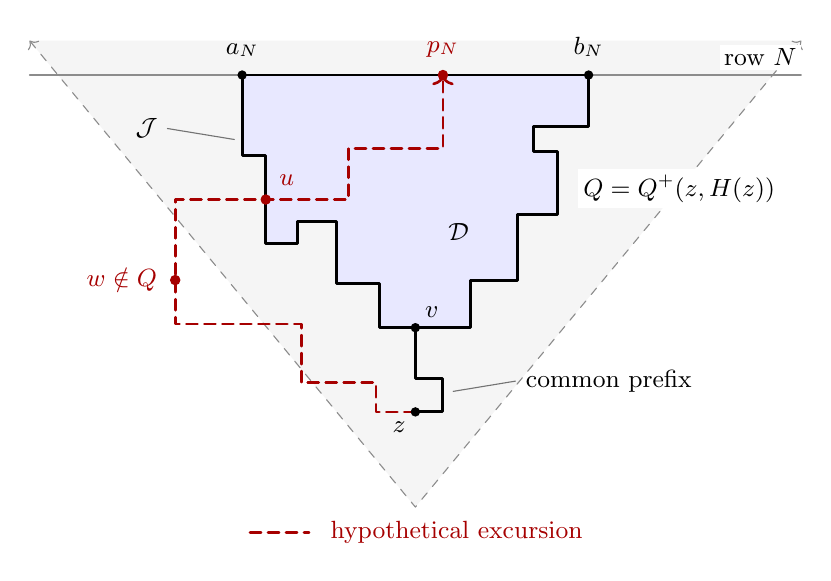
\begin{tikzpicture}[x=1cm,y=.93cm,font=\small,
  line cap=round,line join=round]
  \fill[black!4] (0,-1.3)--(-4.9,5.07)--(4.9,5.07)--cycle;
  \draw[black!45,dashed,<->] (-4.9,5.07)--(0,-1.3)--(4.9,5.07);
  \fill[blue!9!white]
    (0,1.15)--(-.45,1.15)--(-.45,1.75)--(-1,1.75)
    --(-1,2.6)--(-1.5,2.6)--(-1.5,2.3)--(-1.9,2.3)
    --(-1.9,3.5)--(-2.2,3.5)--(-2.2,4.6)
    --(2.2,4.6)--(2.2,3.9)--(1.5,3.9)--(1.5,3.55)
    --(1.8,3.55)--(1.8,2.7)--(1.3,2.7)--(1.3,1.8)
    --(.7,1.8)--(.7,1.15)--cycle;
  \draw[black!45] (-4.9,4.6)--(4.9,4.6);
  \draw[line width=.95pt] (-2.2,4.6)--(2.2,4.6);
  \node[anchor=south east,fill=white,inner sep=1.5pt]
    at (4.9,4.66) {row $N$};

  \draw[line width=1.05pt]
    (0,0)--(.35,0)--(.35,.45)--(0,.45)--(0,1.15);
  \draw[black!55] (1.27,.42)--(.48,.28);
  \node[anchor=west] at (1.28,.42) {common prefix};

  \draw[line width=1.05pt]
    (0,1.15)--(-.45,1.15)--(-.45,1.75)--(-1,1.75)
    --(-1,2.6)--(-1.5,2.6)--(-1.5,2.3)--(-1.9,2.3)
    --(-1.9,3.5)--(-2.2,3.5)--(-2.2,4.6);
  \draw[line width=1.05pt]
    (0,1.15)--(.7,1.15)--(.7,1.8)--(1.3,1.8)
    --(1.3,2.7)--(1.8,2.7)--(1.8,3.55)--(1.5,3.55)
    --(1.5,3.9)--(2.2,3.9)--(2.2,4.6);

  \draw[red!65!black,line width=.95pt,dash pattern=on 4pt off 2.5pt,->]
    (0,0)--(-.5,0)--(-.5,.4)--(-1.45,.4)--(-1.45,1.2)
    --(-3.05,1.2)--(-3.05,2.9)--(-.85,2.9)--(-.85,3.6)
    --(.35,3.6)--(.35,4.6);
  \fill (0,0) circle (1.7pt) (0,1.15) circle (1.7pt)
    (-2.2,4.6) circle (1.7pt) (2.2,4.6) circle (1.7pt);
  \fill[red!65!black] (-3.05,1.8) circle (1.9pt)
    (-1.9,2.9) circle (1.9pt) (.35,4.6) circle (1.9pt);
  \node[below left] at (0,0) {$z$};
  \node[above right] at (0,1.15) {$v$};
  \node[above=3pt] at (-2.2,4.6) {$a_N$};
  \node[above=3pt] at (2.2,4.6) {$b_N$};
  \node[above=3pt,text=red!65!black] at (.35,4.6) {$p_N$};
  \node[left=3pt,text=red!65!black] at (-3.05,1.8) {$w\notin Q$};
  \node[above right=2pt,text=red!65!black] at (-1.9,2.9) {$u$};
  \node at (.55,2.45) {$\mathcal D$};
  \node[fill=white,inner sep=2pt] at (3.35,3.05) {$Q=Q^+(z,H(z))$};
  \draw[black!55] (-3.15,3.87)--(-2.3,3.72);
  \node[left] at (-3.15,3.87) {$\mathcal J$};
  \draw[red!65!black,line width=.95pt,dash pattern=on 4pt off 2.5pt]
    (-2.1,-1.65)--(-1.35,-1.65);
  \node[anchor=west,text=red!65!black] at (-1.2,-1.65)
    {hypothetical excursion};
\end{tikzpicture}
\caption{First-arrival trapping, schematically, in $Q=Q^+(z,H(z))$.
The bounding arcs from the split $v$ to $a_N,b_N$, together with the row
segment, form $\mathcal J$ and enclose $\mathcal D\subset Q$.
The common prefix from $z$ need not lie in $\mathcal D$.
A hypothetical intermediate ray visiting $w$ outside the cone must
contact a bounding arc at $u$ before its first arrival at
$p_N\in(a_N,b_N)$, contradicting finite uniqueness. The dashed excursion
depicts this contradiction; no height monotonicity is assumed.}
\label{fig:trapping}
\end{figure}


Thus every intermediate upper ray is in $Q$.  Rays with an endpoint
label are the unique endpoint rays.  Reflection proves the same
statement for lower rays.  The reasoning was deterministic on the
single event already specified and applied to an arbitrary ray, so it
establishes the simultaneous all-ray assertion.
\end{proof}

\begin{lemma}[Crossing from separated sites]\label{lem:crossing}
Let $x_1<y_1$, and suppose upper rays $p$ from $x$ and $q$ from $y$ satisfy
\[
 p\subset Q^+(x,H_x),\qquad q\subset Q^+(y,H_y).
\]
If
\begin{equation}\label{eq:crossing-separation}
 s(y_1-x_1)>H_x+H_y+|x_2-y_2|
\end{equation}
and $r(\rho_p)>r(\rho_q)$, then the rays intersect.  The same assertion
holds for two lower rays in the corresponding lower cones, with the
horizontal coordinates of their lower labels in place of $r(\rho_p)$
and $r(\rho_q)$.
\end{lemma}

\begin{proof}
For upper rays put $h=\max(x_2,y_2)$.  Both rays have a last visit to
row $h$, because they tend upwards.  Call the two last vertices
$\widehat x,\widehat y$.  The cone bounds give
\[
 |\widehat x_1-x_1|\leq\frac{h-x_2+H_x}{s},\qquad
 |\widehat y_1-y_1|\leq\frac{h-y_2+H_y}{s}.
\]
Since $(h-x_2)+(h-y_2)=|x_2-y_2|$,
\eqref{eq:crossing-separation} implies
$\widehat x_1<\widehat y_1$.  If the rays did not intersect, their
portions from these last visits to their first visits to a sufficiently
high row would be disjoint strip crossings.  Their order there would
remain $p,q$, contradicting \Cref{lem:ray-order} and the strict reverse
order of their labels.  For lower rays use
$h=\min(x_2,y_2)$ and the last visits before departure towards height
$-\infty$.  The same estimates and the lower form of
\Cref{lem:ray-order} apply.
\end{proof}

In particular, the separation required on a common horizontal row is
linear in the sum of the offsets.  Heights differing by a bounded
amount only add that amount to the numerator in
\eqref{eq:crossing-separation}.  For fixed sites $u,v$ and sites
$y=(N,h)$ on any fixed horizontal row, \Cref{prop:cone} gives
$H(y)=o(N)$.  Thus for all sufficiently large $N$ the crossing criterion
applies to every reverse-ordered pair of rays from $u,y$, and also to
every such pair from $v,y$.  This simultaneous choice will be useful
when comparing whole ranges of Busemann values.

\section{Exceptional labels and opposite coalescence}
\label{sec:exceptional}

Fix one of the charts of Lemma~\ref{lem:charts}, with upper label
set $I$ and opposite label set $-I$.  Throughout the deterministic
arguments below, work in an environment satisfying the simultaneous
conclusions of Theorem~\ref{thm:structure}, Lemma~\ref{lem:uniform-metric},
and Proposition~\ref{prop:cone}.  The coalescence assertion in
Theorem~\ref{thm:structure} is only a statement for each fixed label.
We shall obtain the following different statement: every label at which
branching or Busemann nonuniqueness occurs has a coalescing family at its
opposite label.  The exceptional label may depend on the environment.

\Needspace{6\baselineskip}
\subsection{Calibrated rays and countability}

\begin{lemma}[Rays calibrated from an arbitrary vertex]
\label{lem:calibrated-rays}
Let $p$ be a ray, let $B=B_p$, and let $x\in\Z^2$.  There is a ray
$q=(q_j)_{j\ge0}$ from $x$ such that
\begin{equation}
  T(x,q_j)=B(x,q_j)\qquad(j\ge0).
  \label{eq:calibrated-from-x}
\end{equation}
Moreover, $q$ has the same label as $p$.  In general the conclusion
concerns the labels; it does not assert $B_q=B_p$.
\end{lemma}

\begin{proof}
Take the finite geodesics from $x$ to $p_k$.  Since $p$ is simple,
$|p_k|\to\infty$, and their lengths tend to infinity.  Local finiteness
and a diagonal subsequence give a local limit $q$ from $x$.  Each finite
prefix of $q$ is eventually a prefix of these finite geodesics, so $q$
is a simple infinite geodesic.

By Lemma~\ref{lem:busemann-basic},
\begin{equation}
 d_k(x):=T(x,p_k)-B(x,p_k)\ge0,
 \qquad d_k(x)\longrightarrow0.
 \label{eq:calibrated-limit-defect}
\end{equation}
If $w$ lies on the geodesic from $x$ to $p_k$, then
\[
 0\le T(x,w)-B(x,w)
 \le T(x,p_k)-B(x,p_k)=d_k(x),
\]
because $T(w,p_k)\ge B(w,p_k)$.  For each fixed vertex of the local
limit, let $k$ tend to infinity along the chosen subsequence.  This
proves \eqref{eq:calibrated-from-x}.

For any $w\in\Z^2$, the same metric bound and
\eqref{eq:calibrated-from-x} give
\[
 T(x,q_j)-T(w,q_j)
 \le B(x,q_j)-B(w,q_j)=B(x,w).
\]
Consequently $B_q(x,w)\le B(x,w)$.  Write $\sigma=\rho_q$ and
$\rho=\rho_p$.  Asymptotic linearity, with the fixed basepoint $x$,
and the choices $w=ke_i$ and $w=-ke_i$, $i=1,2$, imply respectively
$\sigma(e_i)\le\rho(e_i)$ and $\sigma(e_i)\ge\rho(e_i)$.
Thus $\sigma=\rho$.
\end{proof}

Call a label $\rho\in I$ \emph{exceptional} in an environment $\omega$
if at least one of the following holds:
\begin{enumerate}[label=(\roman*)]
\item two distinct rays of label $\rho$ start at the same vertex;
\item two rays of label $\rho$ have different Busemann functions.
\end{enumerate}
Denote this set by $\mathcal E_I(\omega)$.

\begin{proposition}[Countability of exceptional labels]
\label{prop:exceptional-countable}
Almost surely $\mathcal E_I(\omega)$ is at most countable.  The same
conclusion holds with $I$ replaced by $-I$.
\end{proposition}

\begin{proof}
We prove the two assertions in the definition separately.

\emph{Branching.}
Fix a vertex $x$ and two different first edges $e,f$ incident to $x$.
There are at most two labels in $I$ that are realized both by a ray
from $x$ beginning with $e$ and by one beginning with $f$.  Suppose,
to the contrary, that there are three such labels
$\rho_1,\rho_2,\rho_3$, with
$r(\rho_1)<r(\rho_2)<r(\rho_3)$.  Choose the six corresponding rays.
The geodesics from $x$ form a tree: once two of them diverge, they
cannot meet again, by uniqueness of finite geodesics.  In particular
the two first-edge branches are disjoint away from $x$.

Choose a horizontal row sufficiently high that its six first-arrival
vertices are distinct and have the label order supplied by
Lemma~\ref{lem:ray-order}.  Such a row exists: rays of different
labels have disjoint tails, and rays in the two first-edge branches
never meet away from $x$.  The endpoints occur as three consecutive
groups, one for each label, and each group contains one endpoint of
each branch.  Color the endpoints according to the first edge $e$ or
$f$.  The resulting six-letter word is a concatenation of three
two-letter words, each containing both colors.  It has at least three
changes of color, and hence contains an alternating four-letter
subsequence.

Connect the two $e$-colored endpoints of this subsequence by the
unique arc in the $e$ branch, and connect the two $f$-colored endpoints
by the corresponding arc in the $f$ branch.  Both arcs avoid $x$,
since the two root paths defining each arc share their first edge.
Their interiors are strictly below the chosen row, since all six
root paths were stopped on their first visit to that row.  The arcs
are disjoint, but their endpoints alternate along the row.  This is
impossible: the first arc together with the row segment between its
ends is a Jordan curve, and the second arc must cross it away from
the row.  This proves the claim for $x,e,f$.

Two distinct rays from a common vertex have a first vertex of
divergence.  Applying the preceding claim there, and taking the
countable union over vertices and first-edge pairs, proves
countability for condition~(i).

\emph{Busemann nonuniqueness.}
First consider two vertices $x,y$, with $y$ sufficiently far to the
right of $x$ that the crossing conclusion of
Lemma~\ref{lem:crossing} applies to every pair of upper rays from
these vertices with reversed strict label order.  If $B,B'$ are
Busemann functions of upper rays with labels $\rho,\sigma$ satisfying
$r(\rho)<r(\sigma)$, then
\begin{equation}
 B(x,y)\le B'(x,y).
 \label{eq:ordered-busemann-values}
\end{equation}
Indeed, use Lemma~\ref{lem:calibrated-rays} to take a $B$-calibrated
ray from $y$ and a $B'$-calibrated ray from $x$.  Their labels are
$\rho$ and $\sigma$, respectively, so they intersect at a vertex
$w$.  Calibration at $w$ and the metric bounds on Busemann increments
give
\begin{align*}
 B(x,y)&=B(x,w)-T(y,w)\le T(x,w)-T(y,w)\\
       &\le T(x,w)-B'(y,w)=B'(x,y).
\end{align*}

For such a pair $x,y$, let
\[
 S_\rho(x,y)=\{B_p(x,y):p\text{ is a ray with label }\rho\}.
\]
These sets are bounded by $T(x,y)$ in absolute value.  If
$r(\rho)<r(\sigma)$ and both sets are nonempty,
\eqref{eq:ordered-busemann-values} states that
\begin{equation}
 \sup S_\rho(x,y)\le\inf S_\sigma(x,y).
 \label{eq:ordered-value-ranges}
\end{equation}
Thus the nonempty open intervals
$(\inf S_\rho(x,y),\sup S_\rho(x,y))$ are pairwise disjoint.  Each
contains a rational number, so only countably many labels can have
more than one possible value at this pair.

It remains to ensure that these comparisons detect every possible
disagreement of Busemann functions.  Fix arbitrary vertices $u,v$.
Proposition~\ref{prop:cone} supplies finite offsets controlling all
upper rays from $u$ and from $v$.  For $y_N=(N,0)$ it also supplies
offsets $H_N=o(N)$ controlling all upper rays from $y_N$.  The height
differences between $y_N$ and $u,v$ are fixed.  For all sufficiently
large integers $N$, the horizontal separations therefore dominate
the offsets and height differences as required by
Lemma~\ref{lem:crossing}.  Choose any such $N$.  Both pairs $(u,y_N)$
and $(v,y_N)$ then satisfy \eqref{eq:ordered-value-ranges} for all
labels and all their Busemann functions.

If two upper-ray Busemann functions $B,B'$ of the same label disagree
at $(u,v)$, additivity in
\[
 B(u,v)=B(u,y_N)-B(v,y_N),\qquad
 B'(u,v)=B'(u,y_N)-B'(v,y_N)
\]
forces a disagreement at one of those two comparison pairs.  The
labels producing a disagreement at $(u,v)$ are consequently contained
in a union of two countable sets.  Taking a countable union over
$u,v\in\Z^2$ proves countability for condition~(ii).  The choice of
$N$ may depend on the environment and on $u,v$; it uses the all-ray
cone bounds, and no common rate of Busemann convergence over labels.
Reflection of the vertical coordinate proves the lower-sector
assertion.
\end{proof}

\subsection{Independent environments and exceptional parameters}

The probabilistic use of countability requires care because
$\mathcal E_I$ is random.  We give the measurable argument before
constructing the coupling that will use it.

\begin{lemma}[Countable exceptional parameters in an independent metric]
\label{lem:independent-exceptional}
Let $V,W$ be independent environments, each with the iid law $\PP$.
Almost surely, simultaneously for every $\rho\in\mathcal E_I(V)$,
all $W$-rays of label $-\rho$ coalesce.
\end{lemma}

\begin{proof}
Use the standard Borel configuration space $\Omega$ before completing
its probability measure, and the path space
$\mathcal P=(\Z^2)^{\mathbb N_0}$.  Let
$\mathsf R(\omega,p,\rho)$ be the assertion that $p$ is a simple
nearest-neighbor ray in $\omega$, that all its Busemann limits exist,
and that its Busemann function is asymptotically linear to $\rho$.
For a linear functional $\rho$, this is a Borel relation by
Lemma~\ref{lem:measurable}. Define Busemann evaluations to be zero
where their limits do not exist; the relation $\mathsf R$ explicitly
requires existence.

For paths $p_1,p_2$ satisfying $\mathsf R(\omega,p_i,\rho)$, the
exceptionality witness is the Borel disjunction
\begin{equation}
 \bigl[p_{1,0}=p_{2,0}\ \text{and}\ p_1\ne p_2\bigr]
 \quad\text{or}\quad
 \bigl[\exists x,y\in\Z^2:
 B_{p_1}(x,y)\ne B_{p_2}(x,y)\bigr].
 \label{eq:exceptional-witness-test}
\end{equation}
The common-tail test for paths $q_1,q_2$ is Borel as well:
\begin{equation}
 \exists a,b\in\mathbb N_0\quad
 \forall k\in\mathbb N_0:\ q_{1,a+k}=q_{2,b+k}.
 \label{eq:common-tail-test}
\end{equation}
Its negation tests noncoalescence.

Now define the bad set $J\subset\Omega\times\Omega$ by the existence
of one label $\rho\in I$ and four paths $p_1,p_2,q_1,q_2$ such that
\begin{enumerate}[label=(\alph*)]
\item $\mathsf R(v,p_i,\rho)$ holds for $i=1,2$, and
      \eqref{eq:exceptional-witness-test} holds in $v$;
\item $\mathsf R(w,q_i,-\rho)$ holds for $i=1,2$, and
      \eqref{eq:common-tail-test} fails.
\end{enumerate}
This is directly the projection of a Borel relation on
$\Omega^2\times I\times\mathcal P^4$.  In particular, $J$ is
analytic and is measurable in the completion of $\PP\otimes\PP$.

For every $v$ in the full-measure countability event of
Proposition~\ref{prop:exceptional-countable}, its section is
\begin{equation}
 J_v=\bigcup_{\rho\in\mathcal E_I(v)}
 \{w:\text{two $w$-rays of label $-\rho$ do not coalesce}\}.
 \label{eq:countable-null-section}
\end{equation}
For this fixed $v$, each label in the countable union is an ordinary
fixed parameter.  Symmetry gives $-\rho\in C$, and
Theorem~\ref{thm:structure} makes the corresponding analytic event
in $w$ null.  Hence $\PP(J_v)=0$ for almost every $v$.
Completed-product Fubini gives
$(\PP\otimes\PP)(J)=0$.  Equivalently, replace $J$ by a Borel set
equal to it outside a Borel product-null set and apply ordinary
Fubini; the sections of that null set are null for almost every
$v$.  This argument needs no measurable enumeration of
$\mathcal E_I(v)$.

No universal all-ray condition is inserted into the four-path
relation. Such regularity conditions are imposed outside the
projection, as specified after Lemma~\ref{lem:measurable}.
\end{proof}

\subsection{Transfer across a horizontal cut}

Let $U$ have the iid law.  For $n\ge1$, set
\[
 H_n=\{z\in\Z^2:z_2=-n\},\qquad
 E_n^+=\{\{x,y\}:x\sim y,\ x_2\ge-n,\ y_2\ge-n\}.
\]
Take independent iid replacement arrays $A^{(n)},D^{(n)}$, all
independent of $U$, and define
\begin{equation}
 (V_n)_e=
 \begin{cases}U_e,&e\in E_n^+,\\ A^{(n)}_e,&e\notin E_n^+,\end{cases}
 \qquad
 (W_n)_e=
 \begin{cases}D^{(n)}_e,&e\in E_n^+,\\ U_e,&e\notin E_n^+.\end{cases}
 \label{eq:half-plane-coupling}
\end{equation}
For each $n$, the pair $(V_n,W_n)$ has law $\PP\otimes\PP$: the
coordinates of $U$ retained in its two members are disjoint, and
their replacement coordinates are independent.  Independence of
the pairs for different $n$ is neither asserted nor needed.

We will use $V_n$ to retain the two upper rays witnessing an exceptional
label, with their exact label and any distinguishing Busemann evaluation.
After choosing one such cut, $W_n$ must retain tails of arbitrary rays
with the opposite label, so that Lemma~\ref{lem:independent-exceptional}
can be applied to the independent pair $(V_n,W_n)$.

\begin{lemma}[Half-plane transfer]
\label{lem:cut-transfer}
There is a deterministic increasing sequence $n_k\to\infty$ and an
event of probability one for the coupling
\eqref{eq:half-plane-coupling} with the following properties.
\begin{enumerate}[label=(\roman*)]
\item For every finite collection of upper $U$-rays and every finite
      set $K\subset\Z^2$, all sufficiently large $k$ have the
      following property.  Every ray $p$ in that collection is a
      $V_{n_k}$-ray with exactly its original label, and
      \[
       B_p^{V_{n_k}}(x,y)=B_p^U(x,y)\qquad(x,y\in K).
      \]
      More precisely, for each such $k$ and $p$, the distances
      $T_{V_{n_k}}(x,p_j)$ and $T_U(x,p_j)$ are equal for all
      sufficiently large $j$, simultaneously for $x\in K$.
\item For each fixed $n\ge1$, every lower $U$-ray has a tail which
      is a $W_n$-ray with exactly its original label.
\end{enumerate}
The thresholds may depend on the rays, their labels, $K$, and, in
part~(ii), on $n$.
\end{lemma}

\begin{proof}
First take a common event on which all-ray asymptotics, finite
geodesic existence and uniqueness, and the uniform metric estimate
hold in $U$ and in all $V_n,W_n$.  This is a countable intersection
of events of probability one.

\emph{A single subsequence for the moving cuts.}
For any metric $T$ put
\begin{equation}
 E_n(T)=\sup_{x,y\in\Z^2}
 \frac{|T(x,y)-m(y-x)|}{|x|+|y|+n}.
 \label{eq:moving-metric-error}
\end{equation}
For a fixed typical metric, $E_n(T)\to0$.  Indeed, for any
$\eps>0$, Lemma~\ref{lem:uniform-metric} bounds the numerator by
$\eps(|x|+|y|)$ outside a finite set of pairs.  The maximum error
on the remaining finite set, divided by $n$, tends to zero.  Since
each $V_n$ has the iid law, $E_n(T_{V_n})\to0$ in probability.
Choose an increasing deterministic sequence $n_k$ such that
\[
 \PP\bigl(E_{n_k}(T_{V_{n_k}})>2^{-k}\bigr)<2^{-k}.
\]
After a further probability-one restriction, Borel--Cantelli gives
\begin{equation}
 E_{n_k}(T_{V_{n_k}})\longrightarrow0.
 \label{eq:subsequence-metric-error}
\end{equation}
This is the only subsequence used in the proof.

Fix now an arbitrary upper $U$-ray $p$, with label $\rho\in I$.
Write
\begin{equation}
 a(w)=B_p^U(0,w)-\rho(w)=o(|w|),\qquad
 B_p^U(x,z)=\rho(z-x)+a(z)-a(x).
 \label{eq:rooted-busemann-error}
\end{equation}
All contacts of $\rho$ are strictly upper, so compactness gives
\begin{equation}
 \gamma=\min_{|d|=1,\ d_2\le0}\bigl(m(d)-\rho(d)\bigr)>0.
 \label{eq:opposite-semicircle-gap}
\end{equation}
Let $K$ be finite and enlarge it to contain $p_0$.  Set
$R_K=\max_{x\in K}|x|$.  For $n\ge2R_K+1$, $x\in K$, and
$z\in H_n$, the vector $z-x$ points into the lower half-plane and
\begin{equation}
 |z-x|\ge |z|/2,\qquad
 |x|+|z|+n\le \tfrac52|z|\le5|z-x|.
 \label{eq:moving-cut-comparability}
\end{equation}
For $n=n_k$, \eqref{eq:moving-metric-error} therefore yields
\begin{align}
 T_{V_n}(x,z)-B_p^U(x,z)
 &\ge \gamma|z-x|
      -E_n(T_{V_n})(|x|+|z|+n)-|a(z)|-|a(x)|.
 \label{eq:moving-cut-barrier-estimate}
\end{align}
The metric error is $o(|z-x|)$ uniformly over these $x,z$, by
\eqref{eq:subsequence-metric-error} and
\eqref{eq:moving-cut-comparability}.  The same is true of $|a(z)|$:
$|z|\ge n\to\infty$ uniformly on the cut, and
$|z|\le2|z-x|$.  Finally, the finitely many $|a(x)|$ are bounded.
Thus, for all sufficiently large $k$, uniformly for $x\in K$ and
$z\in H_{n_k}$,
\begin{equation}
 T_{V_{n_k}}(x,z)-B_p^U(x,z)
 \ge \frac\gamma2|z-x|\ge\frac\gamma4 n_k.
 \label{eq:moving-cut-positive-barrier}
\end{equation}
The same estimate holds with $V_{n_k}$ replaced by $U$, because
$E_n(T_U)\to0$.

\emph{The last-cut comparison.}
The heights of $p_j$ tend to $+\infty$, so the entire ray lies
strictly above $H_n$ for all sufficiently large $n$.  If a finite
walk from $x$ to $p_j$, with both endpoints above the cut, visits
$H_n$, let $z$ be its last cut vertex.  Its suffix after $z$ lies
strictly above the cut and uses only edges in $E_n^+$.  Its cost in
$V_n$ is consequently at least
\begin{align}
 T_{V_n}(x,z)+B_p^U(z,p_j)
 &=B_p^U(x,p_j)
   +\bigl[T_{V_n}(x,z)-B_p^U(x,z)\bigr].
 \label{eq:last-cut-lower-bound}
\end{align}
The suffix bound uses only $B_p^U(z,p_j)\le T_U(z,p_j)$ and its
unchanged edge costs.  Repeated visits to the cut and repeated edges
in the walk cause no problem: all occur either in the prefix or in
a suffix whose cost still bounds the corresponding distance.  The
same comparison holds in $U$.

For $x=p_0$, the original segment of $p$ has cost
$B_p^U(p_0,p_j)$ and is unchanged.  By
\eqref{eq:moving-cut-positive-barrier} every cut-touching competitor
is more expensive; a competitor avoiding the cut has its original
$U$ cost.  Hence every prefix of $p$ minimizes in $V_{n_k}$ for all
sufficiently large $k$, and $p$ is a ray there.

For any fixed $x\in K$, \eqref{eq:calibrated-limit-defect}, applied in
$U$, says that
\[
 T_U(x,p_j)-B_p^U(x,p_j)\longrightarrow0.
\]
Fix a sufficiently large $k$.  Eventually this defect is smaller
than $\gamma n_k/4$.  By the $U$ version of
\eqref{eq:last-cut-lower-bound}, a $U$-geodesic to $p_j$ must then
avoid the cut.  It provides an unchanged competitor in $V_{n_k}$.
The $V_{n_k}$ version excludes every cut-touching walk that could
improve that competitor, and every walk avoiding the cut has its
$U$ cost.  It follows that
\begin{equation}
 T_{V_{n_k}}(x,p_j)=T_U(x,p_j)
 \quad\text{for all sufficiently large }j.
 \label{eq:finite-witness-distance-equality}
\end{equation}
Because $K$ is finite, one target-index threshold works for all its
vertices.  Subtracting two such distance equalities and taking the
limit preserves every $B_p(x,y)$ with $x,y\in K$.

\emph{Exact identification of the label at a fixed cut.}
Preservation of a path alone does not identify both coordinates of
its Busemann asymptote.  Fix one $n=n_k$ for which $p$ was preserved,
and henceforth regard $U,V_n$, and the cut as fixed.  Fix $0<c<1$,
take $x$ in the sector $x_2\ge c|x|$, and let $z\in H_n$.  With
$d=z-x$ we have
\[
 |d|\ge x_2+n\ge c|x|,
 \qquad |z|\le|d|+|x|.
\]
Consequently
\begin{equation}
 |z-x|\ge\kappa(|x|+|z|),\qquad
 \kappa=\frac{c}{c+2}>0.
 \label{eq:fixed-cut-comparability}
\end{equation}
This bound holds uniformly along the entire infinite cut, including
cut vertices with arbitrarily large horizontal coordinate.  Since
$d_2<0$, \eqref{eq:opposite-semicircle-gap} gives
\[
 m(d)-\rho(d)\ge\gamma\kappa(|x|+|z|).
\]
For every $\eps>0$ there is $C_\eps<\infty$ such that
$|a(w)|\le\eps|w|+C_\eps$ for every $w$.  The fixed-metric uniform
estimate, separately in $U$ and $V_n$, and
\eqref{eq:rooted-busemann-error} now give, for $|x|$ sufficiently
large in the sector and every $z\in H_n$,
\begin{align*}
 T_{V_n}(x,z)-B_p^U(x,z)
 &\ge (\gamma\kappa-2\eps)(|x|+|z|)-2C_\eps.
\end{align*}
Choose $\eps<\gamma\kappa/8$ and then increase the lower bound on
$|x|$.  In both metrics we obtain the uniform barrier
\begin{equation}
 \min\{T_{V_n}(x,z),T_U(x,z)\}-B_p^U(x,z)
 \ge\frac{\gamma\kappa}{2}(|x|+|z|).
 \label{eq:fixed-cut-positive-barrier}
\end{equation}
In particular, the error at the moving basepoint $x$, as well as
that at $z$, has been included explicitly.

For each such $x$, its calibration defect tends to zero as the
target runs out along $p$.  The last-cut argument just used proves
$T_{V_n}(x,p_j)=T_U(x,p_j)$ for all sufficiently large $j$.
Meanwhile the preserved root $p_0$ satisfies
$T_{V_n}(p_0,p_j)=T_U(p_0,p_j)$ for every $j$, whether or not $p_0$
is in the strict sector.  Thus
\begin{equation}
 B_p^{V_n}(p_0,x)=B_p^U(p_0,x)
 \quad\text{for all sufficiently far }x\text{ with }x_2\ge c|x|.
 \label{eq:sector-busemann-equality}
\end{equation}
Take $c=1/2$, and use first $x=ke_2$ and then
$x=k(e_1+e_2)$.  Dividing \eqref{eq:sector-busemann-equality} by $k$
and using asymptotic linearity in the two fixed environments shows
that their labels agree on $e_2$ and $e_1+e_2$.  These vectors are
independent, so the labels are exactly equal.

All steps so far are pathwise on the common event already chosen.
For a finite collection of rays, apply them to each ray and take
the largest of the finitely many thresholds.  This proves
part~(i), with the stated quantifiers.

\emph{Lower tails for a fixed $W_n$.}
Fix $n$ and an arbitrary lower $U$-ray $q$ of label $\lambda\in-I$.
Use
\begin{gather*}
 a_-(w)=B_q^U(0,w)-\lambda(w)=o(|w|),\\
 \gamma_-=\min_{|d|=1,\ d_2\ge0}(m(d)-\lambda(d))>0.
\end{gather*}
Choose $c\in(0,1/2]$ small enough that eventually
$q_{j,2}\le-c|q_j|$.  This is possible because the limit directions
of $q$ lie in the strict lower sector of the chart.  If
$x_2\le-c|x|$, $|x|\ge2n/c$, and $z\in H_n$, then
\[
 |z-x|\ge c|x|-n\ge\tfrac c2|x|,
 \qquad |x|+|z|\le(1+4/c)|z-x|.
\]
The displacement $z-x$ points upward.  Applying the fixed-metric
uniform estimate to $U,W_n$ and bounding both errors
$a_-(x),a_-(z)$ exactly as above gives, for all sufficiently large
$|x|$ in this lower sector, uniformly for $z\in H_n$,
\begin{equation}
 \min\{T_{W_n}(x,z),T_U(x,z)\}-B_q^U(x,z)
 \ge\frac{\gamma_-c}{2(c+4)}(|x|+|z|).
 \label{eq:lower-fixed-cut-barrier}
\end{equation}
Only the usual uniform estimate in this particular fixed $W_n$ has
been used.

Choose a vertex $a=q_L$ sufficiently far along $q$ that
\eqref{eq:lower-fixed-cut-barrier} applies to $a$ and the whole
remaining tail lies strictly below $H_n$.  For a walk from $a$ to
a later $q_j$ that touches the cut, take its last cut vertex $z$.
After this last visit its first edge goes downward and every later
vertex is strictly below the cut.  Every edge of this suffix is
outside $E_n^+$ and hence is shared by $U$ and $W_n$.  Horizontal
edges on the cut, which are not shared, are part of the prefix.
The analogue of \eqref{eq:last-cut-lower-bound}, now using
\eqref{eq:lower-fixed-cut-barrier}, shows that this walk is more
expensive than the unchanged segment of $q$.  Walks that avoid the
cut have their $U$ costs.  Thus the tail from $a$ is a $W_n$-ray,
and its distances from $a$ to all later $q_j$ are unchanged.

Finally take any sufficiently far $x$ in the strict lower sector.
Its $U$ calibration defect relative to $q_j$ tends to zero, so
\eqref{eq:lower-fixed-cut-barrier} and the last-cut argument give
eventual equality of distances from $x$ in the two environments.
Using the preserved anchor $a$ yields equality of the two tail
Busemann functions at $(a,x)$.  The sequences $x=-ke_2$ and
$x=-k(e_1+e_2)$ belong to this sector for our choice $c\le1/2$.
Asymptotic linearity along them identifies the label of the
$W_n$-tail as exactly $\lambda$.

Since all $W_n$ were included in the initial countable
probability-one event, the argument applies to every fixed $n$ and
every lower ray, with its own tail index.  There is no estimate on
the rate of convergence of the sequence of metrics $W_n$, and no
uniformity of thresholds over labels is required.
\end{proof}

\subsection{The simultaneous conclusion}

\begin{proposition}[Coalescence at opposite exceptional labels]
\label{prop:opposite-coalescence}
Almost surely, simultaneously for all $\rho\in\mathcal E_I(U)$,
every two $U$-rays of label $-\rho$ coalesce.  Almost surely the same
statement holds with upper and lower sectors exchanged.  These
conclusions hold simultaneously for the countable collection of
charts under consideration.
\end{proposition}

\begin{proof}
Use the coupling \eqref{eq:half-plane-coupling}.  For every $n$,
Lemma~\ref{lem:independent-exceptional} applies to $(V_n,W_n)$.
Take their countable intersection, together with the
probability-one event in Lemma~\ref{lem:cut-transfer}.

On this event, fix any $\rho\in\mathcal E_I(U)$ and two upper rays
witnessing its exceptionality.  If they witness branching, their
distinct paths and common starting vertex are preserved by
Lemma~\ref{lem:cut-transfer}(i) for every sufficiently deep
subsequence cut.  If instead they witness different Busemann
functions, choose one pair $x,y$ at which those functions differ
and include $x,y$ in the finite witness set of that lemma.  At
every sufficiently deep subsequence cut the two paths retain both
their exact label $\rho$ and those unequal evaluations.  In either
case choose one such cut $n$; then
$\rho\in\mathcal E_I(V_n)$.

Now let $q,q'$ be any two lower $U$-rays of label $-\rho$.
Lemma~\ref{lem:cut-transfer}(ii), for this fixed $n$, supplies tails
of both which are $W_n$-rays of the same exact label $-\rho$.
They coalesce by the property of $(V_n,W_n)$.  Equality of their
tails is equality of their vertex sequences and thus also means
that the original $U$-rays coalesce.

The argument made arbitrary pathwise choices of $\rho$ and its
witnesses after the common event was fixed.  It therefore proves
the simultaneous assertion in the coupling, and hence for its
$U$ marginal.  Its failure is itself the analytic four-witness
event with both environments set equal to $U$, so it is measurable
in the completed marginal space.  Reflection gives the reversed
statement; a countable intersection gives both statements in all
charts.
\end{proof}

\section{A label budget on horizontal lines}\label{sec:budget}

Fix a chart $I$ from \Cref{lem:charts}, with horizontal order $r$ and
cone slope $s>0$ as in \Cref{prop:cone}. For each deterministic label
$\gamma$ used below, $B_\gamma$ denotes the common Busemann function
of its coalescing family in the base environment.

The comparison concerns a bigeodesic in a finitely increased metric
whose upper label lies between two deterministic labels $\alpha,\beta$
with $r(\alpha)<r(\beta)$.
Suppose the increase adds a total cost $b$ on finite initial portions of
its arms from a site $k$. Under the cone bounds stated below, the base
upper $\alpha$-ray and lower $-\beta$-ray from a sufficiently distant
site $y$ to the right supply a bypass in unchanged weights. We will prove
that
\[
 b\le B_\alpha(y,k)+B_{-\beta}(y,k).
\]
For successive sites whose labels lie in the same interval, these
increments telescope. Their two linear parts leave the width
$r(\beta)-r(\alpha)$ as the available cost per horizontal unit.
We first use this budget in a one-edge resampling estimate needed to
exclude forks, and later to contradict the growing gains constructed in
\Cref{sec:tilts}.

Choose deterministic nested finite sets $D_1\subset D_2\subset\cdots$
of labels in $I$, containing both chart endpoints, such that their union
$D_I$ is dense in $I$ and $r(D_I)$ contains the endpoints of every
complementary interval of $r(I)$ in its convex hull. There are only
countably many such intervals, so these choices are possible. The bins
of $\Pi_j$ are
\[
 (\alpha,\beta)_I
   =\{\rho\in I:r(\alpha)<r(\rho)<r(\beta)\},
\]
where $\alpha,\beta$ are consecutive members of $D_j$ in $r$-order.
Empty bins may be retained. Their widths always sum to
\begin{equation}\label{eq:chart-width}
 W_I=r(\rho_r)-r(\rho_\ell).
\end{equation}
Every two distinct labels of $I\setminus D_I$ eventually belong to
different bins. If a label lies strictly between them, density supplies
an intervening member of $D_I$; otherwise they are endpoints of a
complementary interval and already belong to $D_I$.

By \Cref{cor:fixed-label}, almost surely no bigeodesic has an end label
in the deterministic countable set $D_I\cup(-D_I)$. The same exclusion
and the fixed-functional conclusions of \Cref{thm:structure} hold
simultaneously for all partition endpoints in all charts, and in every
countable collection of environments whose laws are absolutely
continuous with respect to the iid law. We work on the corresponding
common event. Every fixed-label comparator ray is calibrated by its
$B_\gamma$, by \Cref{lem:busemann-basic}.

\begin{lemma}[Comparison after a finite increase]\label{lem:budget-comparison}
Let $T$ be a base metric and $T^k$ a metric obtained by increasing finitely
many edge weights.  Both environments are assumed to have the structural
properties already established.  Suppose that $k,y$ lie on the same
horizontal line, with $k_1<y_1$, and that the following conditions hold for
a bin $(\alpha,\beta)_I$.
\begin{enumerate}[label=\textup{(\roman*)}]
\item Every changed edge has both endpoints in
$\{z:|z-k|_\infty\le R\}$, where $R\ge1$.
\item In $T^k$ there is an oriented bigeodesic through $k$ with upper
label $\rho\in(\alpha,\beta)_I$.  Its arms $p^+$ and $p^-$ are contained
in $Q^+(k,H_p)$ and $Q^-(k,H_p)$, respectively.
\item Finite initial portions of these two arms have all their vertices
in the same ball of radius $R$, and the sum of the increases along those
portions is at least $b>0$.
\item The base rays from $y$ of labels $\alpha$ and $-\beta$ are contained
in $Q^+(y,H_c)$ and $Q^-(y,H_c)$, respectively.
\end{enumerate}
There is a separation $S=S(s,R,H_p,H_c)$ such that $y_1-k_1>S$ implies
\begin{equation}\label{eq:budget-comparison}
 b\le B_\alpha(y,k)+B_{-\beta}(y,k).
\end{equation}
One may take
\begin{equation}\label{eq:budget-separation}
 S=\max\left\{R+\frac{R+H_c}{s},\frac{H_p+H_c}{s}\right\}
 \le C_s(1+R+H_p+H_c),
\end{equation}
with $C_s$ depending only on $s$.  In particular, the choice
of $S$ is uniform over bins and does not depend on the magnitudes of the
individual increases.
\end{lemma}

\begin{proof}
Put $d=y_1-k_1$.  If a vertex $w$ belongs to the ball of radius $R$ about
$k$, then
\[
 |w_2-y_2|\le R,
 \qquad |w_1-y_1|\ge d-R.
\]
Membership in either comparator cone would therefore require
$R\ge s(d-R)-H_c$.  Thus
\begin{equation}\label{eq:avoid-gain-ball}
 d>R+\frac{R+H_c}{s}
\end{equation}
makes both base comparator rays avoid the entire ball.  Their edge
weights are unchanged in $T^k$.  Since every other edge weight only
increases, each comparator remains a geodesic ray in $T^k$.
\Cref{lem:finite-change} preserves its label.

Increase the separation further, if necessary, to apply
\Cref{lem:crossing} with offsets $H_p,H_c$.  The upper marked ray is to
the left at its starting site but has label strictly east of $\alpha$.
The same ordering holds for the lower rays, since
\[
 r(-\beta)=-r(\beta)<-r(\rho)=r(-\rho).
\]
The upper comparator therefore meets $p^+$, and the lower comparator
meets $p^-$.  Call intersection vertices $w^+$ and $w^-$, respectively.
By \eqref{eq:avoid-gain-ball}, each intersection is outside the ball.
Consequently it occurs after the whole prescribed initial gain portion
of the corresponding marked arm.  This remains true if an arm leaves
and later reenters the ball, since every vertex of its prescribed initial
portion lies in the ball.

Let $g^+$ and $g^-$ be the increases on those portions, so
$g^++g^-\ge b$.  Writing $\operatorname{cost}_T$ for the cost of a
specified finite path in the base weights, domination by passage time and
then by a Busemann increment gives
\[
 \begin{split}
 \operatorname{cost}_{T^k}(p^+[k,w^+])
 &\ge g^++\operatorname{cost}_T(p^+[k,w^+])
 \ge g^++B_\alpha(k,w^+),\\
 \operatorname{cost}_{T^k}(p^-[k,w^-])
 &\ge g^-+\operatorname{cost}_T(p^-[k,w^-])
 \ge g^-+B_{-\beta}(k,w^-).
 \end{split}
\]
The marked segment from $w^-$ through $k$ to $w^+$ is minimizing in
$T^k$.  A competing finite walk follows the lower comparator backwards
from $w^-$ to $y$, then follows the upper comparator to $w^+$.
The cost of this walk in $T^k$ equals its base cost, namely
\[
 B_{-\beta}(y,w^-)+B_\alpha(y,w^+).
\]
No disjointness between the two comparator portions is required: a finite
walk is an admissible competitor and its cost counts every traversal.
Comparison with the marked segment yields
\[
 b+B_\alpha(k,w^+)+B_{-\beta}(k,w^-)
 \le B_\alpha(y,w^+)+B_{-\beta}(y,w^-).
\]
Additivity cancels the increments ending at the intersection vertices
and gives exactly \eqref{eq:budget-comparison}.  Both the avoidance bound
and the separation in \Cref{lem:crossing} have the asserted dependence
on the offsets and $R$.
\end{proof}

\Needspace{4\baselineskip}
\begin{proposition}[The label budget]\label{prop:label-budget}
Fix a bin $(\alpha,\beta)_I$, an integer spacing $l\ge1$, and a gain
$b>0$.  On a common probability space, mark some sites of the horizontal
grid $k_j=(jl,0)$, $j\in\Z$.  Suppose all sites have the same marginal
probability $q_{\alpha,\beta}$ of being marked in this bin, and the base
environment has its usual fixed-label Busemann asymptotics.  Suppose also
that for successive marks $k<y$ in the bin the comparison
\eqref{eq:budget-comparison} holds.  In particular, this is so if the
hypotheses of \Cref{lem:budget-comparison} hold with common deterministic
bounds and successive marks are sufficiently separated.  Then
\begin{equation}\label{eq:label-budget}
 \frac{b}{l}\,q_{\alpha,\beta}
 \le r(\beta)-r(\alpha).
\end{equation}
No independence or ergodicity assumption on the marks is needed.
\end{proposition}

\begin{proof}
Set $w=r(\beta)-r(\alpha)>0$ and, for $j\ge0$, write
\[
 A_j=B_\alpha(0,k_j)+B_{-\beta}(0,k_j)
     =-wjl+e_j.
\]
The sign in this formula uses
$\alpha(e_1)+(-\beta)(e_1)=r(\alpha)-r(\beta)=-w$.
The two fixed-label asymptotics give $e_j=o(jl)$ as $j\to\infty$.
Define
\[
 E_N=\max_{0\le j\le N}|e_j|.
\]
Then $E_N/(Nl)\to0$ almost surely.  To see the needed uniformity, for
each $\delta>0$ choose $J$ so that $|e_j|\le\delta jl$ when $j\ge J$.
The earlier errors have a finite maximum $C_J$, and
$E_N\le\max\{C_J,\delta Nl\}$.  Let $N\to\infty$ and then
$\delta\downarrow0$.  This argument controls random first and last marks
without replacing them by deterministic endpoints.

Let $m_N$ be the number of marks in $\{k_0,\ldots,k_N\}$.  If
$m_N\ge2$, list their indices as $i_1<\cdots<i_{m_N}$.  Summing the
comparison over consecutive marks and using additivity gives
\[
 \begin{split}
 b(m_N-1)
 &\le A_{i_1}-A_{i_{m_N}}\\
 &=wl(i_{m_N}-i_1)+e_{i_1}-e_{i_{m_N}}
 \le wNl+2E_N.
 \end{split}
\]
If $m_N=0$ or $1$, the same upper bound applies to
$b(m_N-1)_+$.  Therefore, in all cases,
\begin{equation}\label{eq:bounded-budget-count}
 bm_N\le b+wNl+2E_N,
 \qquad
 \limsup_{N\to\infty}\frac{m_N}{Nl}\le\frac wb
 \quad\text{almost surely}.
\end{equation}
The expectation step uses only the deterministic bounds
\[
 0\le\frac{m_N}{Nl}\le\frac{N+1}{Nl}\le\frac2l,
 \qquad N\ge1.
\]
Fatou's lemma applied to the nonnegative variables
$2/l-m_N/(Nl)$ gives the bounded reverse Fatou inequality
\[
 \limsup_{N\to\infty}\EE\frac{m_N}{Nl}
 \le\EE\left[\limsup_{N\to\infty}\frac{m_N}{Nl}\right]
 \le\frac wb.
\]
Equal marginal probabilities imply
$\EE m_N=(N+1)q_{\alpha,\beta}$ by linearity of expectation.  Hence
$q_{\alpha,\beta}/l\le w/b$, as asserted.  In particular, this proof
takes no expectation of either a Busemann error or a Busemann increment.
\end{proof}

We now prepare the one-edge resampling estimate. Replacing an edge by
an independent sample keeps the output environment iid. Choosing the old
weight below one level and the replacement above a larger level creates
a fixed positive gain. The same thresholds will ensure that long simple
paths contain many edges above the larger level. These edges supply the
edge--label credits in the fork count and the accumulated gains in the
later perturbations.

\begin{lemma}[Usable edges on long simple paths]\label{lem:usable}
There exist $a_0<b_0$ such that
\begin{equation}\label{eq:low-usable-probabilities}
 \begin{gathered}
 p_a=\PP(t_e\le a_0)>0,
 \qquad q=\PP(t_e<b_0)<\frac1{64},\\
 p_b=\PP(t_e\ge b_0)=1-q>0.
 \end{gathered}
\end{equation}
Call an edge \emph{usable} if $t_e\ge b_0$, and put
$\theta=8\sqrt q<1$.  For each vertex $x$ and integer $n_0\ge1$,
\begin{equation}\label{eq:usable-fixed-site}
 \PP\left(
 \begin{array}{c}
 \text{some simple path from $x$ of length $j\ge n_0$}\\
 \text{has fewer than $j/2$ usable edges}
 \end{array}\right)
 \le\frac{\theta^{n_0}}{1-\theta}.
\end{equation}
If $U_n$ is the event that every simple path starting in
$[-3n,3n]^2\cap\Z^2$ and having length at least $n/2$ has at least half
its edges usable, then
\begin{equation}\label{eq:usable-box}
 \PP(U_n^c)
 \le (6n+1)^2\frac{\theta^{\lceil n/2\rceil}}{1-\theta}
 \longrightarrow0.
\end{equation}
Almost surely, at every fixed vertex all sufficiently long simple paths
satisfy the same fraction bound.
\end{lemma}

\begin{proof}
Let $a$ be the bottom of the support of $G$.  It is finite, and
$G(\{a\})=0$.  As $b\downarrow a$ with $b>a$, the probability
$G([0,b))$ tends to zero and is positive.  Choose $b_0>a$ so that this
probability is less than $1/64$, and choose $a_0\in(a,b_0)$.
The definition of $a$ gives $p_a>0$, proving
\eqref{eq:low-usable-probabilities}.

The edges of a simple path are distinct.  For a specified path of length
$j$, independence and a union bound over subsets of its edges bound the
probability that at least $j/2$ of them are unusable by
\[
 2^j q^{j/2}.
\]
This also bounds the probability of fewer than $j/2$ usable edges.
There are at most $4^j$ nearest-neighbor paths of length $j$ from a given
vertex, so the union bound over simple paths is at most $\theta^j$.
Summing over $j\ge n_0$ proves \eqref{eq:usable-fixed-site}; the further
union bound over the $(6n+1)^2$ starting vertices proves
\eqref{eq:usable-box}.  Finally, the events in
\eqref{eq:usable-fixed-site} decrease as $n_0\to\infty$, and their
probabilities tend to zero.  Countability gives the last assertion
simultaneously at all vertices.  These estimates use no moment of an
individual edge weight.
\end{proof}

For an edge $e=\{x,x+v\}$, where $v$ is a lattice unit vector, and
$H\ge1$, let $\mathcal R_e(H)$ be the following regularity event in the
environment under consideration: from each endpoint $z$ of $e$, every
ray with label in $I$ is contained in $Q^+(z,H)$, and every ray with label
in $-I$ is contained in $Q^-(z,H)$.  Set $N_e(H)=0$ if $e$ is unusable
or $\mathcal R_e(H)$ fails.  Otherwise define
\begin{equation}\label{eq:edge-label-count-definition}
 N_e(H)=\#\{\rho\in I:\text{$e$ lies on a bigeodesic of upper label $\rho$}\}.
\end{equation}
Here the count is the number of distinct labels, and is assigned the
value $\infty$ if the set is infinite.  This convention does not
presuppose that the label set is countable.  By \Cref{lem:measurable},
existence of finitely many distinct witnessing labels is measurable in
the completed space.  The universal regularity event is imposed as a
separate environment-only filter; it is not inserted into an
existential path projection.

\begin{proposition}[Expected label count at an edge]\label{prop:edge-count}
There is a finite constant $C$, depending only on the chart and the weight
law, such that for every lattice edge $e$ and every $H\ge1$,
\begin{equation}\label{eq:edge-label-count}
 \EE N_e(H)\le C(H+1).
\end{equation}
\end{proposition}

\begin{proof}
Fix a unit vector $v$ and let $e_k=\{k,k+v\}$ for sites $k$ on a
horizontal grid whose spacing will be chosen below.  Use one iid base
environment $t$ and independent samples $\widehat t_{e_k}$ with law
$G$.  The individual environment $t^k$ equals $t$ off $e_k$ and equals
$\widehat t_{e_k}$ on $e_k$.  Each individual environment has precisely
the iid law.  We take the common full-measure event for the base and all
these countably many individual environments, including the fixed-label
exclusions at every endpoint in $D_I$ and $-D_I$.

For a bin $(\alpha,\beta)_I$, let $A_e^{\alpha,\beta}(H)$ denote the
event in an iid environment that $e$ is usable, $\mathcal R_e(H)$ holds,
and a bigeodesic whose upper label is in this bin uses $e$.  Mark $k$ in
this bin when
\begin{equation}\label{eq:one-edge-mark}
 t_{e_k}\le a_0
 \quad\text{and}\quad
 A_{e_k}^{\alpha,\beta}(H)\text{ holds in }t^k.
\end{equation}
The original variable $t_{e_k}$ is independent of the entire individual
environment $t^k$: that environment consists of the independent sample
$\widehat t_{e_k}$ and the other base coordinates.  Consequently the
common marginal marking probability is exactly
\begin{equation}\label{eq:one-edge-mark-probability}
 q_{\alpha,\beta}
   =p_a\,\PP\bigl(A_e^{\alpha,\beta}(H)\bigr),
\end{equation}
where $e$ is any fixed translate of $\{0,v\}$.
The regularity test is measurable in the individual environment, so it
does not alter this independence calculation.  Dependence between marks
at different sites is immaterial.

On a marking event, the one changed edge is increased by at least
$b_0-a_0$.  Every witnessing bigeodesic passes through $k$, and the edge
$e_k$ is the first edge of one of its arms based there.  Use that edge as
the gain portion of that arm and use the empty portion of the other arm.
Thus the modification and both gain portions fit in a ball of radius
one, and the total gain is at least
\[
 b=b_0-a_0>0.
\]
The regularity event in $t^k$ confines both marked arms with offset $H$.

We must also establish confinement of the \emph{base} comparator rays at
every marked site; base regularity was not assumed in
\eqref{eq:one-edge-mark}.  Let $q$ be any base ray from $k$ with label in
$I$ or $-I$.  A simple path from $k$ can traverse $e_k$ only as its first
edge.  Indeed, a later traversal in either direction would revisit $k$.
If $q$ avoids $e_k$, all its weights are unchanged and it remains a ray
in $t^k$ by monotonicity.  Its label is unchanged by
\Cref{lem:finite-change}, so $\mathcal R_{e_k}(H)$ in $t^k$ puts it in
the appropriate cone at $k$.

If $q$ uses $e_k$ first, its tail from $k+v$ avoids $e_k$ and remains a
ray in $t^k$, with the same label.  That tail lies in the corresponding
cone at $k+v$ with offset $H$.  For either choice of sign, the inequality
\[
 \pm(w_2-k_2-v_2)\ge s|w_1-k_1-v_1|-H
\]
implies
\[
 \pm(w_2-k_2)
 \ge s|w_1-k_1|-\bigl(H+|v_2|+s|v_1|\bigr).
\]
Including the initial vertex $k$, and then the initial edge by convexity,
confines the whole base ray with offset at most $H+1+s$.
This proves the needed base comparator control at both fixed labels
$\alpha$ and $-\beta$, uniformly over all bins.  It explains why
regularity was required at both endpoints of $e_k$.

Choose an integer grid spacing $l=l(H)$ large enough for
\Cref{lem:budget-comparison} with $R=1$, $H_p=H$, and $H_c=H+1+s$.
It may be chosen so that
\begin{equation}\label{eq:one-edge-spacing}
 2\le l(H)\le C_0(H+1)
\end{equation}
for a chart-dependent constant $C_0$, uniformly in the unit vector $v$.
The lower bound makes the edges $e_k$ at distinct grid sites distinct.
Any two different marked sites are now sufficiently separated.  Applying
\Cref{prop:label-budget} and
\eqref{eq:one-edge-mark-probability} to each bin yields
\[
 \PP\bigl(A_e^{\alpha,\beta}(H)\bigr)
 \le\frac{l(H)}{(b_0-a_0)p_a}
       \bigl(r(\beta)-r(\alpha)\bigr).
\]
For the finite partition $\Pi_j$, let $K_j(e,H)$ count its occupied bins
among the labels counted by $N_e(H)$.  Linearity of expectation and
\eqref{eq:chart-width} give
\begin{equation}\label{eq:occupied-bin-bound}
 \EE K_j(e,H)
 \le\frac{l(H)W_I}{(b_0-a_0)p_a}.
\end{equation}

On the event excluding $D_I$ as bigeodesic labels, refinement never loses a
counted label, so $K_j(e,H)$ is nondecreasing.  Every finite collection of
distinct counted labels is eventually in distinct bins.  Thus
\[
 K_j(e,H)\uparrow N_e(H),
\]
also when the latter is infinite: apply the separation assertion to
arbitrarily large finite collections.  Monotone convergence in
\eqref{eq:occupied-bin-bound}, followed by \eqref{eq:one-edge-spacing},
proves \eqref{eq:edge-label-count}.  Translation invariance and the
finite number of edge directions give one constant for all $e$.
\end{proof}

\section{Excluding forks and identifying Busemann pairs}\label{sec:forks}

The finite-tree count in this section follows the density-versus-boundary
principle of Burton and Keane~\cite{BurtonKeane1989}. Here the preceding
label budget bounds the edge--label pairs supplied by distinct branches.

Continue with the fixed chart $I$.  An \emph{upper fork at $x$} consists
of two bigeodesics, oriented toward upper labels in $I$, with the same
upper label, coincident backwards from $x$, and with different first
edges forwards from $x$.  Equivalently, one may require a common
backwards tail and a split at $x$: uniqueness of finite geodesics from a
vertex on that common tail identifies the two paths up to their split.
A lower fork is defined with the orientation reversed.  These are
existence events with two path witnesses and a label witness, and hence
are measurable in the completed space by \Cref{lem:measurable}.

\begin{proposition}[Absence of forks]\label{prop:no-forks}
Almost surely there is no upper or lower fork in any of the countably
many charts under consideration.
\end{proposition}

\begin{proof}
The counting argument groups forks by label and extracts disjoint
forward branches within each group. Positive fork density would force
a cubic expected number of usable edge--label pairs in large boxes;
uniform confinement and \Cref{prop:edge-count} give an arbitrarily small
cubic upper bound.

It suffices first to exclude upper forks in one chart.  Work on the
simultaneous event of \Cref{prop:opposite-coalescence}.  Every upper fork
label is exceptional by the first test in
\Cref{prop:exceptional-countable}, since two different rays of that label
start at its split vertex.  Consequently all lower rays with the
opposite label coalesce, simultaneously for every label arising in this
way.  In particular, a finite collection of bigeodesics with one such
upper label has a common backwards tail.  A vertex sufficiently far
along that common tail is a common past root for the entire finite
collection.

Let $F_n$ be the number of vertices in $[-n,n]^2\cap\Z^2$ that are upper
forks for this chart, and let
\[
 p_{\mathrm{fork}}=\PP(0\text{ is an upper fork for this chart}).
\]
The chart and the fork definition are translation invariant, so
\begin{equation}\label{eq:fork-count-mean}
 0\le F_n\le(2n+1)^2,
 \qquad \EE F_n=(2n+1)^2p_{\mathrm{fork}}.
\end{equation}
Fix $\eps>0$ and put $H_n=\lceil\eps n\rceil$.  Let $G_n$ be the
intersection of the event $U_n$ in \Cref{lem:usable} and the event that
$\mathcal R_e(H_n)$ holds for every edge with both endpoints in
$[-2n,2n]^2$.  Uniform all-ray confinement in \Cref{prop:cone} gives
the latter event eventually almost surely: all its endpoint sites lie in
a box of radius a fixed multiple of $n$, and their required offsets are
$o(n)$.  Therefore, for this fixed $\eps$,
\begin{equation}\label{eq:fork-good-event}
 \PP(G_n^c)\longrightarrow0.
\end{equation}
No rate uniform in $\eps$ is asserted or needed.

We claim the following deterministic counting inequality on $G_n$, for
$n\ge2$:
\begin{equation}\label{eq:fork-edge-credit}
 \frac n4 F_n
 \le\sum_{\substack{e:\text{both endpoints in }[-2n,2n]^2}}
          N_e(H_n).
\end{equation}
Choose a witnessing pair at each of the finitely many fork sites counted
by $F_n$, and group the choices according to their exact upper label.
These finite choices are only used to prove a pathwise inequality; no
measurable enumeration of labels is required.

Consider a group containing $q\ge1$ distinct fork sites.  There are at
most $2q$ witnessing bigeodesics in this group.  Their lower rays
coalesce by \Cref{prop:opposite-coalescence}.  Pairwise coalescence of a
finite collection gives a common tail by going beyond all their finitely
many merging locations.  Choose a vertex $o$ on this tail, earlier than
every selected split, and orient each witness forwards from $o$ toward
its upper end.

The union of these forward paths is a rooted tree.  To justify this
directly, the initial path from $o$ to any vertex $z$ on a witness is a
finite geodesic.  If two witnesses visit $z$, finite uniqueness makes
their entire paths from $o$ to $z$ equal.  They therefore cannot diverge
and later meet, and common edges cannot carry conflicting forward
orientations.  Each visited vertex other than $o$ has one parent, and
the resulting graph has no cycle.

Let $\mathcal T$ be the finite subtree obtained by taking the union of
the root paths to the two selected children immediately after every
selected split.  Each of the $q$ split vertices has at least two children
in $\mathcal T$.  For any finite rooted tree with $L$ leaves,
\begin{equation}\label{eq:finite-tree-leaves}
 L-1=\sum_{u:\,d^+_{\mathcal T}(u)>0}
               \bigl(d^+_{\mathcal T}(u)-1\bigr),
\end{equation}
where $d^+_{\mathcal T}(u)$ is its number of children.  Indeed, the sum of
the outdegrees is the number of edges, one less than the number of
vertices; subtracting the number of nonleaves gives
\eqref{eq:finite-tree-leaves}.  Thus $L\ge q+1$.

Every leaf of $\mathcal T$ is an endpoint of one of the root-to-child
paths defining $\mathcal T$.  Otherwise a defining path containing that
leaf would continue to another vertex of $\mathcal T$, contradicting its
being a leaf.  In particular, every leaf is a selected child of a fork
site, and hence lies in $[-n-1,n+1]^2$.  The root paths are allowed to
leave and reenter both boxes; only their terminal children determine this
location of the leaves.  Selected split vertices may also be ancestors
of one another, but each is still a distinct vertex with at least two
children and contributes at least one to
\eqref{eq:finite-tree-leaves}.

For each leaf choose a witnessing bigeodesic containing its defining
root-to-child path, and continue forwards along that witness.  These
continuations are pairwise vertex disjoint.  In fact, if two met at $w$,
uniqueness of the finite geodesic from $o$ to $w$ would put both leaves
on a single root path.  They would be comparable in the ancestor order,
contrary to being distinct leaves of $\mathcal T$.  The same reasoning
rules out an intersection between one continuation and the root path to
another leaf: its own leaf would then be an ancestor of the other one.
An intersection with an earlier point of its own root path contradicts
simplicity.  These conclusions hold throughout the plane, including
parts of $\mathcal T$ outside either box.

Each leaf has infinity-norm distance at least $n-1$ from the boundary of
$[-2n,2n]^2$.  Its continuation eventually reaches this boundary, since
an upper ray in the chart has height tending to $+\infty$.  Stop the
continuation at its first boundary visit.  The resulting path is simple,
all its edges have both endpoints in the outer box, and its length is at
least $n-1\ge n/2$.  Its starting point is in $[-3n,3n]^2$, so $U_n$
supplies at least half its edges as usable.  It therefore supplies at
least $n/4$ usable edges inside the outer box.  Every such edge lies on
the witnessing bigeodesic and satisfies $\mathcal R_e(H_n)$ on $G_n$.
It contributes the group's label to $N_e(H_n)$.

For this group the leaf continuations are disjoint, so no edge is
credited twice with that label.  Groups with different labels credit
different pairs $(e,\rho)$, even if they use the same geometric edge.
Thus the count is of distinct edge--label pairs.  Summing over the groups
credits at least
\[
 \frac n4\sum_{\text{groups}}L
 \ge\frac n4\sum_{\text{groups}}q
 =\frac n4 F_n
\]
pairs, proving \eqref{eq:fork-edge-credit}.

We now take expectations, retaining the scale of the bad-event loss.
By \eqref{eq:fork-count-mean},
\[
 \EE[F_n\mathbf 1_{G_n}]
 \ge (2n+1)^2
       \bigl(p_{\mathrm{fork}}-\PP(G_n^c)\bigr).
\]
The loss after multiplication by $n/4$ is at most
\begin{equation}\label{eq:fork-bad-event-loss}
 \frac n4(2n+1)^2\PP(G_n^c)=o(n^3)
 \qquad\text{for fixed }\eps.
\end{equation}
There are $2(4n)(4n+1)\le40n^2$ edges with both endpoints in the outer
box.  From \eqref{eq:fork-edge-credit} and \Cref{prop:edge-count},
\begin{equation}\label{eq:fork-expectation-bound}
 \frac n4(2n+1)^2
       \bigl(p_{\mathrm{fork}}-\PP(G_n^c)\bigr)
 \le 40C n^2\bigl(\lceil\eps n\rceil+1\bigr).
\end{equation}
Divide by $n^3$ and let $n\to\infty$ for this fixed $\eps$.  Equations
\eqref{eq:fork-good-event} and \eqref{eq:fork-expectation-bound} yield
$p_{\mathrm{fork}}\le40C\eps$.  Sending $\eps\downarrow0$ gives
$p_{\mathrm{fork}}=0$.  Countability of vertices excludes every upper
fork in this chart almost surely.  Reversing upper and lower gives the
same conclusion for lower forks, and the countable union over charts
proves the proposition.
\end{proof}

\begin{corollary}[Common Busemann pairs for a common label]
\label{cor:same-busemann}
On one event of probability one, whenever two oriented bigeodesics $p,q$
in any fixed chart have the same upper label, their two Busemann
functions agree:
\begin{equation}\label{eq:same-busemann-pair}
 B_{p^+}=B_{q^+},\qquad B_{p^-}=B_{q^-}.
\end{equation}
This assertion is simultaneous over the bigeodesics and their possibly
random labels.  It also holds almost surely in every environment whose
law is absolutely continuous with respect to the iid law, and
simultaneously for a countable collection of such environments.
\end{corollary}

\begin{proof}
Take the common full-measure event of
\Cref{prop:opposite-coalescence,prop:no-forks} and the structural
properties.  Let the two bigeodesics have upper label $\rho$.  If their
upper Busemann functions differ, $\rho$ passes the second exceptional
label test of \Cref{prop:exceptional-countable}.  The simultaneous
conclusion of \Cref{prop:opposite-coalescence} makes their lower rays
coalesce.  Choose a vertex $o$ sufficiently far along their common lower
tail.  The forward portions from $o$ are upper geodesic rays.  They
cannot have the same tail, since tail invariance in
\Cref{lem:busemann-basic} would make their upper Busemann functions
equal.  They must therefore have a first split.  Finite uniqueness
prevents any later meeting, so this split is an upper fork with a common
past, contrary to \Cref{prop:no-forks}.

If the lower Busemann functions differ, the lower label $-\rho$ is
exceptional by the same second test.  Apply
\Cref{prop:opposite-coalescence} with upper and lower reversed to
coalesce the upper rays.  Reversing the preceding argument then produces
a forbidden lower fork.  This proves both equalities in
\eqref{eq:same-busemann-pair}.

All these deductions are pathwise on the stated common event.  They do
not take an uncountable union of fixed-label null events, nor assert
coalescence of every one-sided family at random labels.  Absolute
continuity transfers the event to each individual changed environment;
countable intersection gives the final assertion.
\end{proof}

\section{Finite perturbations with divergent gain}\label{sec:tilts}

Fix a chart $I$, its slope $s>0$, and the partitions $\Pi_j$ from
Section~\ref{sec:budget}.  In this section suppose that, for some deterministic
$H_0\geq1$, the following event in an iid environment has probability $p>0$:
there is a bigeodesic through $0$ whose upper label belongs to $I$, avoids
all partition endpoints, and whose two arms lie in $Q^\pm(0,H_0)$.
Denote this event by $\mathcal B(0)$, and its horizontal translate to
$k=(k_1,0)$ by $\mathcal B(k)$.  The chart, $s$, $H_0$, and $p$ remain fixed
throughout the construction.  The eventual proof of \Cref{thm:main} will
reduce a positive probability of bigeodesics to precisely this situation.

We shall obtain, for every positive integer $M$, marks of probability
bounded below independently of $M$.  A mark comes with a bigeodesic in a
finite upward perturbation of the iid environment and a gain of at least
$M$ on an initial portion of that bigeodesic.  A second requirement, a
strictly raised edge within a fixed number $R_0$ of steps, will prevent
two marks on a suitably spaced horizontal grid from having the same
label.  The distinction between this fixed $R_0$ and the larger radius
needed for the gain $M$ is essential.

\subsection{A shared family of finite perturbations}

Bates and Chatterjee~\cite[Lemmas~2.3--2.4]{BatesChatterjee2020}
bound the change of product law for small Bernoulli replacements whose
distributions have bounded density relative to the original law.
The low-to-high replacement below is a monotone instance of this
construction; related spatially varying passage-time perturbations
appear in \cite[Section~2.3]{DembinElboimPeled}.
We derive its estimates directly, share the edge samples between sites,
and compute the conditional law given an individual modified environment.

Use the thresholds $a_0<b_0$ of \Cref{lem:usable}, and write
\[
 p_a=G([0,a_0])>0,\qquad p_b=G([b_0,\infty))>0,
 \qquad g=b_0-a_0>0.
\]
Thus $q=G([0,b_0))$ satisfies $8\sqrt q<1$.  An edge is usable when its
weight is at least $b_0$. Write $\mu=G^{\mathcal E}$ for the iid law of
the base environment; probability $\PP$ below is taken on the enlarged
coupling. Take, independently for every edge $e$, a triple
$(X_e,U_e,Z_e)$, where
\[
 X_e\sim G,\qquad U_e\sim\operatorname{Unif}[0,1],\qquad
 Z_e\sim G(\,\cdot\mid[b_0,\infty)).
\]
The coordinates of each triple are independent, as are the triples at
different edges.  The base environment is $X=(X_e)_e$, with metric $T$.
All variants below use these same triples.

For an edge $e$ with endpoints $w,w'$, put
\[
 h(e)=\max\{|w_2|,|w'_2|\},\qquad
 \delta_h=\frac{\eta}{(h+2)\log(h+2)},\quad h\geq0,
\]
where $\eta>0$ will be chosen shortly, independently of $M$.  Require
$\delta_0\leq p_a/2$, and define
\begin{equation}\label{eq:shared-raise}
 \xi_e=\mathbf1\{X_e\leq a_0,\ U_e\leq\delta_{h(e)}/p_a\},
 \qquad
 \widehat X_e=
 \begin{cases}
 Z_e,&\xi_e=1,\\
 X_e,&\xi_e=0.
 \end{cases}
\end{equation}
In particular $\widehat X_e\geq X_e$, and
$\widehat X_e-X_e\geq g$ whenever $\xi_e=1$.

For a horizontal site $k=(k_1,0)$ and an integer $R\geq1$, define the
finite set of edges
\begin{equation}\label{eq:tilt-region}
 A_k(R)=\left\{e:\ h(e)\leq R,\quad
  \max_{w\text{ endpoint of }e}|w_1-k_1|
       \leq1+\frac{h(e)+H_0}{s}\right\}.
\end{equation}
Let $Y^{k,R}$ equal $\widehat X_e$ on $A_k(R)$ and $X_e$ elsewhere,
and denote its metric by $T^{k,R}$.  For two horizontal sites $k,y$,
let $Y^{k,y,R}$ instead use $\widehat X_e$ on
$A_k(R)\cup A_y(R)$, with metric $T^{k,y,R}$.  In an overlap there is
one use of the same sample $\widehat X_e$.  We never apply the replacement
operation twice to an edge.

The absolute height in \eqref{eq:tilt-region} accommodates excursions in
either vertical direction.  Indeed, if a bigeodesic through $k$ has its
arms in $Q^\pm(k,H_0)$, then every vertex $w$ of either arm satisfies
\begin{equation}\label{eq:whole-path-width}
 s|w_1-k_1|\leq |w_2|+H_0.
\end{equation}
For the upper arm this follows from
$s|w_1-k_1|\leq w_2+H_0$, and for the lower arm from
$s|w_1-k_1|\leq-w_2+H_0$.  Consequently every edge of this bigeodesic
with $h(e)\leq R$ belongs to $A_k(R)$.  In particular its first $R$
upper-arm edges belong to this set: the $j$th edge has $h(e)\leq j$.

\begin{lemma}[Uniform change of law]\label{lem:likelihood}
Every individual environment $Y^{k,R}$ and every union environment
$Y^{k,y,R}$ has law absolutely continuous with respect to $\mu$.
There is a finite constant $C$, depending only on $s,H_0,p_a,p_b$, such
that the density $L_{k,R}=d\mathcal L(Y^{k,R})/d\mu$ satisfies
\begin{equation}\label{eq:likelihood-bound}
 \EE_\mu L_{k,R}^2\leq\exp(C\eta^2),\qquad
 \|\mathcal L(Y^{k,R})-\mu\|_{\mathrm{TV}}
 \leq\tfrac12\sqrt{\exp(C\eta^2)-1}.
\end{equation}
The bounds are uniform in $k$ and $R$.
\end{lemma}

\begin{proof}
The law of $\widehat X_e$, for $h(e)=h$, has density relative to $G$
\begin{equation}\label{eq:one-edge-density}
 \lambda_h(t)=1-\frac{\delta_h}{p_a}\mathbf1_{[0,a_0]}(t)
                 +\frac{\delta_h}{p_b}\mathbf1_{[b_0,\infty)}(t).
\end{equation}
The two indicated sets are disjoint.  Direct integration gives
$\int\lambda_h\,dG=1$ and
\begin{align}
 \int\lambda_h^2\,dG
 &=p_a(1-\delta_h/p_a)^2
    +p_b(1+\delta_h/p_b)^2+1-p_a-p_b\notag\\
 &=1+(p_a^{-1}+p_b^{-1})\delta_h^2.
 \label{eq:one-edge-second-moment}
\end{align}
For any deterministic finite set of replaced edges, independence of the
triples makes the full density the product of these one-edge densities;
the exterior has its original iid law.  This proves absolute continuity
for both the individual and union environments.

To bound the product for an individual region, let $N_h$ count its edges
of height $h$.  At positive height $h$, horizontal edges lie in the two
rows of heights $h,-h$, and vertical edges lie in the two strips adjoining
those rows toward height zero.  Each row or strip contains at most
$2(1+(h+H_0)/s)+1$ admissible edges.  At height zero there is only one
horizontal row.  Thus, for example,
\[
 N_h\leq c_s(h+H_0+1),\qquad c_s=12+8/s.
\]
It follows from \eqref{eq:one-edge-second-moment} that
\begin{align*}
 \EE_\mu L_{k,R}^2
 &=\prod_{e\in A_k(R)}
       \bigl[1+(p_a^{-1}+p_b^{-1})\delta_{h(e)}^2\bigr]\\
 &\leq\exp\left\{
 c_s(p_a^{-1}+p_b^{-1})\eta^2
 \sum_{h=0}^{\infty}
 \frac{h+H_0+1}{(h+2)^2\log^2(h+2)}\right\}.
\end{align*}
The series is finite; its terms of leading order are
$1/(h\log^2h)$.  It defines the required constant $C$.
Finally, since $\EE_\mu L_{k,R}=1$, Cauchy--Schwarz gives
\[
 \|\mathcal L(Y^{k,R})-\mu\|_{\mathrm{TV}}
 =\tfrac12\EE_\mu|L_{k,R}-1|
 \leq\tfrac12\sqrt{\EE_\mu L_{k,R}^2-1}.
\]
All modified sets are finite.  The infinite series has been used only
to bound these finite products uniformly.
\end{proof}

Fix $\eta>0$ sufficiently small that $\delta_0\leq p_a/2$ and the total
variation bound in \eqref{eq:likelihood-bound} is at most $p/8$.
This choice is henceforth fixed.

\subsection{The posterior law after selecting a path}

\begin{lemma}[Conditioning on an individual output]\label{lem:posterior}
Fix $k,R$.  Conditional on the entire individual environment $Y^{k,R}$,
the variables $(\xi_e:e\in A_k(R))$ are independent Bernoulli variables
with respective success probabilities
\begin{equation}\label{eq:posterior}
 \theta_e(Y^{k,R}_e)
 =\mathbf1_{[b_0,\infty)}(Y^{k,R}_e)
       \frac{\delta_{h(e)}}{p_b+\delta_{h(e)}}.
\end{equation}
The assertion includes conditioning on every unchanged exterior edge.
If a simple path is selected measurably from this individual output
alone, the same product law holds on any of its finite prefixes lying
in $A_k(R)$, once that prefix is fixed by the conditioning.
\end{lemma}

\begin{proof}
For $e\in A_k(R)$, put $Y_e=\widehat X_e$ and $h=h(e)$.
As measures in $t$, the construction gives
\begin{align}
 \PP(\xi_e=1,Y_e\in dt)
    &=\frac{\delta_h}{p_b}\mathbf1_{[b_0,\infty)}(t)G(dt),
       \label{eq:posterior-joint-one}\\
 \PP(\xi_e=0,Y_e\in dt)
    &=\left[1-\frac{\delta_h}{p_a}\mathbf1_{[0,a_0]}(t)\right]G(dt).
       \label{eq:posterior-joint-zero}
\end{align}
For the first identity multiply the low-input probability $p_a$, the
replacement probability $\delta_h/p_a$, and the conditional law of
$Z_e$.  In the second identity the original sample is retained, except
for the removed mass on $[0,a_0]$.  Dividing the first density by their
sum \eqref{eq:one-edge-density} proves \eqref{eq:posterior}.

The pairs $(\xi_e,Y_e)$ are independent across $A_k(R)$.  Hence their
conditional kernel given the finite output vector is the product of
the kernels just computed.  The entire collection of exterior outputs
$(Y^{k,R}_e:e\notin A_k(R))=(X_e:e\notin A_k(R))$ is independent of
the inside triples.  Testing the product kernel against bounded
functions of finitely many exterior coordinates therefore preserves
the conditional-expectation identity.  A monotone-class argument extends
it to the sigma-field of all exterior coordinates.  This establishes
the claimed law given the full environment.

For the last assertion, the path space is standard Borel.  A selector
measurable in the completion of the output law has a Borel version under
that law.  Given the full output, a finite prefix of this version is a
fixed list of distinct edges.  Restricting the product kernel to that
list proves the assertion.  One can equally partition by the countably
many possible finite prefixes to verify the conditional identity.
No output at another site is included in this conditioning.
\end{proof}

Choose a deterministic $n_0$ so large that the event
\[
 \mathcal U_{n_0}(k)=
 \left\{\begin{array}{l}
 \text{every simple path from $k$ of each length $d\geq n_0$}\\
 \text{has at least $d/2$ usable edges}
 \end{array}\right\}
\]
has iid failure probability at most $p/8$. This follows directly from
\eqref{eq:usable-fixed-site} in \Cref{lem:usable}, whose geometric tail
tends to zero. In particular this condition requires no moment of a
single edge weight.

Write
\[
 \mathcal E_{k,R}=
 \{Y^{k,R}\in\mathcal B(k)\cap\mathcal U_{n_0}(k)\}.
\]
The total variation estimate implies, uniformly in $k,R$,
\begin{equation}\label{eq:output-good-probability}
 \PP(\mathcal E_{k,R})
 \geq p-p/8-p/8\geq p/2.
\end{equation}
By \Cref{lem:measurable} select a witnessing oriented bigeodesic and its
upper label using $Y^{k,R}$ alone.  Use the same selection rule at the
origin and at its horizontal translates.  More explicitly, select in
the completed iid space on $\mathcal B(0)$ and replace the selector by
a Borel version there.  Absolute continuity makes this version valid
almost surely under every individual output law; countably many
translates and radii can be handled simultaneously.  On
$\mathcal E_{k,R}$ the usable-prefix condition is already determined by
the output, and the selected witness satisfies it.  It therefore adds
no information when applying \Cref{lem:posterior}.

\begin{lemma}[Divergent gain along selected prefixes]\label{lem:divergent-gain}
There is a fixed integer $R_0\geq n_0$ such that, for each positive
integer $M$, one can choose a deterministic $R(M)\geq R_0$ with the
following property.  On $\mathcal E_{k,R(M)}$, conditional on
$Y^{k,R(M)}$, with probability at least $3/4$ the selected upper arm has
both a strict raise among its first $R_0$ edges and total increase at
least $M$ along its first $R(M)$ edges.
\end{lemma}

\begin{proof}
Fix an output in $\mathcal E_{k,R}$, and denote the successive edges of
the selected upper arm by $e_1,e_2,\ldots$.  For $j\leq R$ they belong
to $A_k(R)$ and have $h(e_j)\leq j$, as shown in
\eqref{eq:whole-path-width}.  Put
\[
 a_j=\mathbf1\{Y^{k,R}_{e_j}\geq b_0\},\quad
 A_d=\sum_{j=1}^d a_j,\quad
 N_d=\sum_{j=1}^d\xi_{e_j},\quad
 \mu_d=\EE(N_d\mid Y^{k,R}).
\]
The $a_j$ and the selected edges are fixed under this conditioning, and
$A_d\geq d/2$ for every $d\geq n_0$.  The decreasing sequence
$f_j=((j+2)\log(j+2))^{-1}$ satisfies
\begin{equation}\label{eq:gain-mean}
 \mu_d\geq\gamma\sum_{j=1}^d a_jf_j,
 \qquad \gamma=\frac{\eta}{p_b+\delta_0}>0,
 \qquad d\leq R.
\end{equation}
Indeed each usable edge contributes the probability in
\eqref{eq:posterior}, at least $\eta f_j/(p_b+\delta_0)$.
Summation by parts, followed by the prefix bounds, gives for $d\geq n_0$
\begin{align}
 \sum_{j=1}^d a_jf_j
 &=A_df_d+\sum_{j=1}^{d-1}A_j(f_j-f_{j+1})\notag\\
 &\geq\frac12\left[df_d+
          \sum_{j=n_0}^{d-1}j(f_j-f_{j+1})\right]\notag\\
 &=\frac12\left[n_0f_{n_0}+\sum_{j=n_0+1}^df_j\right].
 \label{eq:abel-gain}
\end{align}
The last expression tends to infinity.  Let $m_d$ be $\gamma$ times
this expression, a deterministic increasing lower bound for $\mu_d$.

The selected path is simple, so \Cref{lem:posterior} gives
\begin{equation}\label{eq:gain-variance}
 \operatorname{Var}(N_d\mid Y^{k,R})
   =\sum_{j=1}^d\theta_{e_j}(1-\theta_{e_j})\leq\mu_d.
\end{equation}
Choose $R_0\geq n_0$ with $m_{R_0}\geq8$.  For every $R\geq R_0$,
Chebyshev's inequality gives
\[
 \PP(N_{R_0}=0\mid Y^{k,R})\leq\mu_{R_0}^{-1}\leq1/8.
\]
This choice is independent of $R$ and of the requested gain $M$.
For that gain put $K_M=\lceil M/g\rceil$, and choose $R=R(M)\geq R_0$
so large that $m_R\geq\max\{2K_M,32\}$.  Again by Chebyshev,
\[
 \PP(N_R<K_M\mid Y^{k,R})
 \leq\frac{\mu_R}{(\mu_R-K_M)^2}
 \leq\frac4{\mu_R}\leq\frac18.
\]
At least $K_M$ successful raises give total increase at least
$gK_M\geq M$ on the prefix.  The union bound for the two failure events
proves the stated probability $3/4$.
\end{proof}

\begin{proposition}[Marks with an arbitrary toll]\label{prop:tilt-marks}
With $R_0$ fixed as above, for every positive integer $M$ the common
coupling defines marks $J_M(k)\in\{0,1\}$ at all horizontal sites, with
the same marginal probability at each site and
\begin{equation}\label{eq:initial-mark-probability}
 \PP(J_M(k)=1)\geq p/4.
\end{equation}
A mark selects a bigeodesic $p_k$ in $T^{k,R(M)}$ through $k$, with
upper label $\rho_k\in I$ avoiding all partition endpoints.  Its arms
lie in $Q^\pm(k,H_0)$.  Its first $R(M)$ upper-arm edges have total
increase at least $M$ over the base environment, and one of its first
$R_0$ upper-arm edges has increase at least $g$.
All changes occur in a deterministic bounded neighborhood of $k$ whose
radius may depend on $M$.
\end{proposition}

\begin{proof}
Take $R=R(M)$ from \Cref{lem:divergent-gain}.  On $\mathcal E_{k,R}$
use the already selected path, and mark when both success requirements
of that lemma hold.  Together with \eqref{eq:output-good-probability},
the lemma gives marking probability at least $(p/2)(3/4)=3p/8$, proving
\eqref{eq:initial-mark-probability}.  All the asserted path properties
are part of the selection or the marking test.  The region
$A_k(R)$ lies in a ball about $k$ of radius at most
\begin{equation}\label{eq:defect-radius}
 D_R=R+1+(R+H_0)/s,
\end{equation}
and the prescribed gain portion lies in the ball of radius $R$.

Horizontal translations preserve the distribution of the triples and
their height indices.  Since the selection rule and all tests are
translated in the same way, the marks have equal marginals; in fact this
construction is stationary under horizontal translations.  Marks at
different sites may be dependent.
\end{proof}

The conditional product law has now served its purpose.  Subsequent
filters may depend on the base environment or on other marks and hence
may bias the latent variables $\xi_e$.  We will use the unconditional
bound \eqref{eq:initial-mark-probability} after those filters, without
reapplying \Cref{lem:posterior}.

\subsection{Union metrics and distinct labels}
\label{sec:unions}

Before selecting a pair of marks, fix the common full-measure event
needed for all comparisons.  There are countably many integer radii,
horizontal lattice sites, and pairs of these sites.  By
\Cref{lem:likelihood}, each corresponding individual or union environment
has law absolutely continuous with respect to $\mu$.  Thus almost surely
the base and every one of these environments satisfy the structural
properties, \Cref{lem:opposite}, and the simultaneous conclusion
\Cref{cor:same-busemann}.  They also exclude bigeodesic labels in the
deterministic countable set of partition endpoints.  Intersect these
events with the countably many full-measure events needed for the
selectors and conditional estimates.  In the rest of the argument we
work on this common event.  A subsequently selected random pair of sites
and random label therefore require no additional fixed-label null-event
assertion.

Choose an integer grid spacing $l$, once and for all, satisfying
\begin{equation}\label{eq:fixed-grid-spacing}
 l>R_0+1+\frac{R_0+H_0}{s},
\end{equation}
and restrict marks to $\Lambda=\{(jl,0):j\in\Z\}$.  This spacing is
independent of $M$.

\begin{lemma}[Preservation in a union]\label{lem:union}
Fix $M$, put $R=R(M)$, and suppose distinct sites $k,y\in\Lambda$ are
marked.  Their selected paths $p_k,p_y$ are bigeodesics in the union
metric $T^*=T^{k,y,R}$.  Every edge of $p_k$ has the same weight there
as in $T^{k,R}$, and every edge of $p_y$ has the same weight there as in
$T^{y,R}$.  Their labels are preserved.  Moreover, any raised edge among
the first $R_0$ upper-arm edges of $p_y$ lies outside $A_k(R)$ and has
its base weight in $T^{k,R}$.
\end{lemma}

\begin{proof}
For each edge of $p_k$ of height at most $R$,
\eqref{eq:whole-path-width} puts both endpoints within the width bound
of $A_k(R)$.  Its individual weight is already $\widehat X_e$, so passage
to the union leaves that weight unchanged.  For an edge of greater
height neither region changes its base weight.  This proves the
edgewise assertion along all of $p_k$, including any initial upper-arm
excursion below row zero or lower-arm excursion above it.  The same
argument applies to $p_y$.  All other weights weakly increase in passing
from either individual environment to the union.  Every segment of its
selected bigeodesic therefore still minimizes: its cost is unchanged
and no competitor becomes cheaper.

Only finitely many edges differ between an individual environment and
the union.  The sum of their finite increases bounds the change of any
passage distance, by comparison along a simple minimizing path in the
smaller metric.  The labels of the retained rays are consequently
unchanged by \Cref{lem:finite-change}.

If $e$ belongs to the first $R_0$ edges of $p_y$, both its endpoints
satisfy $|w_1-y_1|\leq R_0$ and $h(e)\leq R_0$.  For every such endpoint,
\[
 |w_1-k_1|\geq |y_1-k_1|-R_0
 >1+(R_0+H_0)/s\geq1+(h(e)+H_0)/s,
\]
where \eqref{eq:fixed-grid-spacing} was used.  Thus $e\notin A_k(R)$.
If it is raised in $T^{y,R}$, its increase in the union over $T^{k,R}$
is at least $g$.  Such an edge cannot lie on $p_k$: every edge of $p_k$
in this height slab already belongs to $A_k(R)$.
\end{proof}

The shared samples and the protected near edge are illustrated in
\Cref{fig:union}.
\begin{figure}[tbp]
\centering
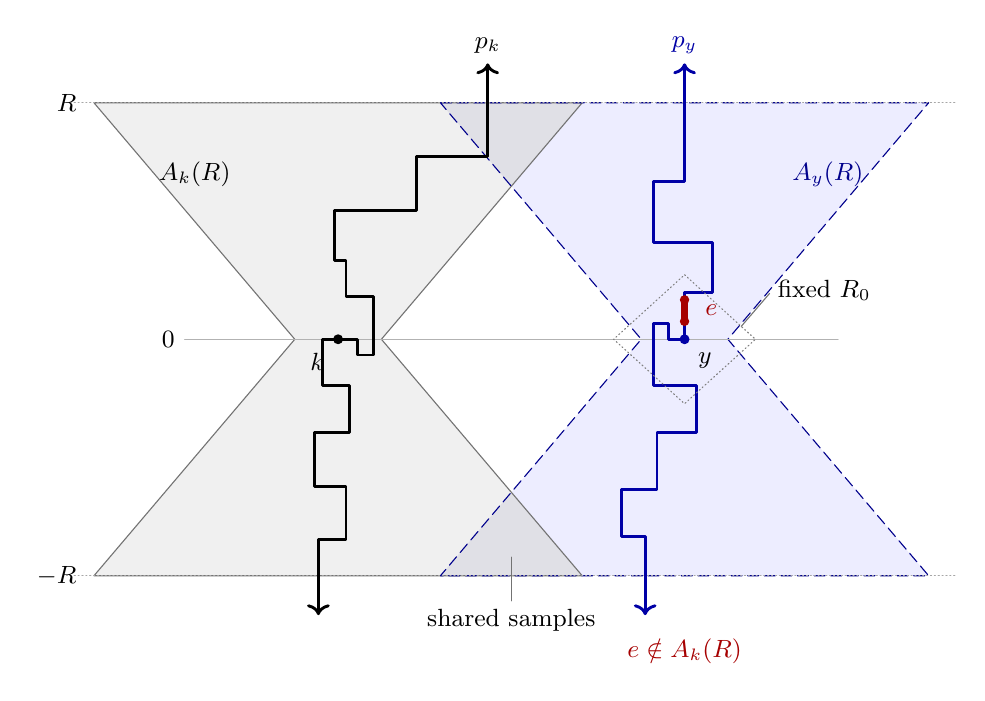
\begin{tikzpicture}[x=1cm,y=.91cm,font=\small,
  line cap=round,line join=round]
  \fill[black!6] (-5.3,3.3)--(.9,3.3)--(-1.65,0)
    --(.9,-3.3)--(-5.3,-3.3)--(-2.75,0)--cycle;
  \fill[blue!7!white] (-.9,3.3)--(5.3,3.3)--(2.75,0)
    --(5.3,-3.3)--(-.9,-3.3)--(1.65,0)--cycle;
  \fill[blue!18!black!12] (0,2.1353)--(.9,3.3)--(-.9,3.3)--cycle;
  \fill[blue!18!black!12] (0,-2.1353)--(.9,-3.3)--(-.9,-3.3)--cycle;
  \draw[black!55] (-5.3,3.3)--(.9,3.3)--(-1.65,0)
    --(.9,-3.3)--(-5.3,-3.3)--(-2.75,0)--cycle;
  \draw[blue!55!black,dash pattern=on 4pt off 2pt]
    (-.9,3.3)--(5.3,3.3)--(2.75,0)
    --(5.3,-3.3)--(-.9,-3.3)--(1.65,0)--cycle;
  \draw[black!35,densely dotted] (-5.65,3.3)--(5.65,3.3);
  \draw[black!35,densely dotted] (-5.65,-3.3)--(5.65,-3.3);
  \draw[black!30] (-4.15,0)--(4.15,0);
  \node[left] at (-5.4,3.3) {$R$};
  \node[left] at (-5.4,-3.3) {$-R$};
  \node[left] at (-4.15,0) {$0$};
  \node at (-4.02,2.3) {$A_k(R)$};
  \node[text=blue!55!black] at (4.02,2.3) {$A_y(R)$};

  \draw[line width=1.05pt,->]
    (-2.2,0)--(-1.95,0)--(-1.95,-.22)--(-1.75,-.22)
    --(-1.75,.6)--(-2.1,.6)--(-2.1,1.1)--(-2.25,1.1)
    --(-2.25,1.8)--(-1.2,1.8)--(-1.2,2.55)--(-.3,2.55)
    --(-.3,3.85);
  \draw[line width=1.05pt,->]
    (-2.2,0)--(-2.4,0)--(-2.4,-.65)--(-2.05,-.65)
    --(-2.05,-1.3)--(-2.5,-1.3)--(-2.5,-2.05)
    --(-2.1,-2.05)--(-2.1,-2.8)--(-2.45,-2.8)--(-2.45,-3.85);
  \draw[blue!65!black,line width=1.05pt,->]
    (2.2,0)--(2.2,.65)--(2.55,.65)--(2.55,1.35)
    --(1.8,1.35)--(1.8,2.2)--(2.2,2.2)--(2.2,3.85);
  \draw[blue!65!black,line width=1.05pt,->]
    (2.2,0)--(2,0)--(2,.22)--(1.8,.22)--(1.8,-.65)
    --(2.35,-.65)--(2.35,-1.3)--(1.85,-1.3)
    --(1.85,-2.1)--(1.4,-2.1)--(1.4,-2.75)
    --(1.7,-2.75)--(1.7,-3.85);
  \node[above] at (-.3,3.85) {$p_k$};
  \node[above,text=blue!65!black] at (2.2,3.85) {$p_y$};
  \fill (-2.2,0) circle (1.8pt);
  \fill[blue!65!black] (2.2,0) circle (1.8pt);
  \node[below left=2pt] at (-2.2,0) {$k$};
  \node[below right=2pt] at (2.2,0) {$y$};

  \draw[black!50,densely dotted] (2.2,.9)--(3.1,0)
    --(2.2,-.9)--(1.3,0)--cycle;
  \draw[red!65!black,line width=2.5pt] (2.2,.25)--(2.2,.55);
  \fill[red!65!black] (2.2,.25) circle (1.7pt)
    (2.2,.55) circle (1.7pt);
  \node[right=4pt,text=red!65!black] at (2.2,.4) {$e$};
  \draw[black!55] (3.28,.64)--(2.92,.18);
  \node[anchor=west] at (3.26,.68) {fixed $R_0$};
  \draw[black!55] (0,-3.65)--(0,-3.04);
  \node at (0,-3.92) {shared samples};
  \node[text=red!65!black] at (2.2,-4.35) {$e\notin A_k(R)$};
\end{tikzpicture}
\caption{Schematic envelopes of the truncated edge regions $A_k(R)$
and $A_y(R)$, not their exact lattice footprints. Overlap uses the same
raised sample for each edge, with no repeated increase. Every marked-path
edge in the slab belongs to its own region, so the union preserves both
paths' weights and geodesic property. The strictly raised edge $e$ lies
among the first $R_0$ steps from $y$ and outside $A_k(R)$ at sufficiently
large fixed separation. The near radius $R_0$ and this separation remain
fixed as $R$ grows.}
\label{fig:union}
\end{figure}

\newpage

\begin{proposition}[No repeated marked label]\label{prop:distinct-marks}
Almost surely, for each positive integer $M$, the selected upper labels
at distinct marked sites of $\Lambda$ are distinct.
\end{proposition}

\begin{proof}
Work on the common event specified above.  Suppose two marked sites
$k\ne y$ have $\rho_k=\rho_y$.  By \Cref{lem:union} both selected
bigeodesics persist with this label in $T^*=T^{k,y,R}$, where $R=R(M)$.
By \Cref{cor:same-busemann} their upper and lower Busemann functions in
this metric agree; denote the common pair by $B^+,B^-$.  For a vertex
$u$ on $p_y$, the bigeodesic inequality of \Cref{lem:opposite}, based
first at $k$ on $p_k$ and then at $u$ on $p_y$, gives
\[
 B^+(k,u)+B^-(k,u)\leq0,\qquad
 B^+(u,k)+B^-(u,k)\leq0.
\]
Additivity and antisymmetry therefore imply
\begin{equation}\label{eq:equal-sum-increments}
 B^+(k,u)+B^-(k,u)=0\qquad(u\in p_y).
\end{equation}

Take a raised edge $e=\{u,v\}$ among the first $R_0$ upper-arm edges of
$p_y$, and orient it toward the upper end, from $u$ to $v$.  Write $t_e^*$
for its weight in the union.  Calibration along the bigeodesic gives
\begin{equation}\label{eq:near-edge-calibration}
 B^+(u,v)=T^*(u,v)=t_e^*.
\end{equation}
Here the last equality holds because the one-edge segment of $p_y$
is itself minimizing.

Let $x_N^-,x_N^+$ tend respectively to the lower and upper ends of
$p_k$, with $k$ between them.  Set
\[
 L_N^*=T^*(x_N^-,u)+t_e^*+T^*(v,x_N^+),\qquad
 D_N^*=T^*(x_N^-,x_N^+).
\]
This $L_N^*$ is the cost of an admissible finite walk, so
$L_N^*\geq D_N^*$.  As $p_k$ is a bigeodesic,
$D_N^*=T^*(x_N^-,k)+T^*(k,x_N^+)$.  The signs in the Busemann definition
then give, separately,
\begin{align*}
 T^*(x_N^-,u)-T^*(x_N^-,k)&\longrightarrow-B^-(k,u),\\
 T^*(v,x_N^+)-T^*(k,x_N^+)&\longrightarrow-B^+(k,v).
\end{align*}
It follows that
\begin{align}
 L_N^*-D_N^*
 &\longrightarrow -B^-(k,u)-B^+(k,v)+t_e^*\notag\\
 &=-\bigl[B^-(k,u)+B^+(k,u)\bigr]-B^+(u,v)+t_e^*=0,
 \label{eq:detour-excess}
\end{align}
by \eqref{eq:equal-sum-increments} and \eqref{eq:near-edge-calibration}.

Choose minimizing finite approach paths in $T^*$ from $x_N^-$ to $u$
and from $v$ to $x_N^+$, and join them by the specified traversal
$u\to v$ of $e$.  Call this finite walk $W_N$.  The approach paths
may intersect each other, the selected bigeodesics, or $e$ itself;
its cost is $L_N^*$ with every traversal counted.
By \Cref{lem:union}, the weight of $e$ in $T^{k,R}$ is its base weight
$X_e$.  Thus
\[
 \Delta=t_e^*-X_e\geq g>0.
\]
On returning from $T^*$ to $T^{k,R}$ every traversal weakly decreases
in cost, and the named middle traversal decreases by $\Delta$.
Consequently
\begin{equation}\label{eq:walk-saving}
 \operatorname{cost}_{T^{k,R}}(W_N)\leq L_N^*-\Delta.
\end{equation}
Any further traversal of the same edge can only increase this saving.
On the other hand, the segment of $p_k$ between $x_N^-$ and $x_N^+$
has cost $D_N^*$ in both metrics, again by \Cref{lem:union}.
For sufficiently large finite $N$, \eqref{eq:detour-excess} gives
$L_N^*-D_N^*<\Delta$.  Then \eqref{eq:walk-saving} makes $W_N$ strictly cheaper in
$T^{k,R}$ than that segment, a contradiction.  This is a pathwise
argument for every marked pair on the common event, and hence proves
the assertion simultaneously for the countably many $M$.
\end{proof}

\section{The final comparison and proof of the theorem}\label{sec:conclusion}

\begin{proof}[Proof of \Cref{thm:main}]
Suppose bigeodesics exist with positive probability.  Each bigeodesic
contains a lattice vertex.  Countability of the vertices and the charts
in \Cref{lem:charts}, together with the exclusion of their deterministic
exceptional labels, yields a chart in which a bigeodesic through some
fixed vertex has positive probability.  Translate that vertex to zero
and use the lattice coordinates of the chart.  By \Cref{prop:cone}, its
arms are contained in $Q^\pm(0,H)$ for some finite $H$ almost surely.
Taking the countable union over integer $H$ gives a deterministic
$H_0\geq1$ for which the event $\mathcal B(0)$ in \Cref{sec:tilts} has
probability $p>0$.  Removing the countably many deterministic partition
endpoints does not change this probability, by the fixed-label
backward-finiteness assertion in \Cref{thm:structure}.

Apply \Cref{prop:tilt-marks} for each positive integer $M$, with the
fixed spacing $l$ from \eqref{eq:fixed-grid-spacing}.  We next impose
two filters on its marks.  The first supplies the base comparator rays
required for \Cref{lem:budget-comparison}; the second supplies their
required separation within each bin.

For a horizontal site $k$, let $\mathcal R_K(k)$ be the event that, in
the unchanged base environment, every ray from $k$ with label in $I$
lies in $Q^+(k,K)$ and every ray from $k$ with label in $-I$ lies in
$Q^-(k,K)$.  By \Cref{prop:cone},
\[
 \mu(\mathcal R_K(k)^c)\longrightarrow0\qquad(K\longrightarrow\infty).
\]
Choose one deterministic $K\geq1$, independent of $M$, such that this
failure probability is at most $p/8$.  It is the same at all horizontal
sites by translation invariance.  Retain a mark when
\[
 \widetilde J_M(k)=J_M(k)\mathbf1_{\mathcal R_K(k)}=1.
\]
Unconditional subtraction, without any independence assertion, gives
\begin{equation}\label{eq:retained-mark-probability}
 q_M:=\PP(\widetilde J_M(k)=1)
 \geq\PP(J_M(k)=1)-\mu(\mathcal R_K(k)^c)
 \geq p/8.
\end{equation}
This filter is imposed after selecting the paths.  Its complement has
an existential ray witness, so $\mathcal R_K(k)$ is a universally
measurable environment event by \Cref{lem:measurable}.  It remains a
separate filter; it is not placed inside an existential path projection.
In particular no new alternation of path quantifiers is used to define
the selected marks.  The translated rule continues to give equal
marginals along the grid.

The near radius $R_0$, spacing $l$, and comparator offset $K$ are fixed
independently of $M$. For each $M$ we choose $R(M)$ and the comparison
separation below, refine the partition, and only then increase $M$.
Fix $M$ for the moment. Its radius $R(M)$ is a fixed finite number.
The selected arms have offset $H_0$, the base comparator rays have
offset $K$, the changed region has radius at most $D_{R(M)}$ from
\eqref{eq:defect-radius}, and the prescribed gain portion has radius at
most $R(M)$.  The comparison in \Cref{lem:budget-comparison} therefore
holds at a finite deterministic horizontal separation $S(M)$.  The same
$S(M)$ works for every bin of every partition $\Pi_j$: the cone bounds
control all the relevant comparator labels in the chart, and the
geometric bounds on the changed region and gain portion are independent
of the bin.  Increase $S(M)$ if necessary to be nonnegative.  Its possible
growth with $M$ has no effect on the already fixed grid spacing $l$.

For the finite partition $\Pi_j$, retain a site with
$\widetilde J_M(k)=1$ only if there is no other site $y$ with
$\widetilde J_M(y)=1$ and
\[
 0<|y-k|\leq S(M)
\]
whose selected label lies in the same bin as $\rho_k$.  Here $k,y$ lie
on the horizontal grid, so the displayed distance is their horizontal
separation.  Denote this final indicator by $J_{M,j}(k)$ and its common
marginal probability by $q_{M,j}$.  The test concerns at most
$2\lfloor S(M)/l\rfloor$ other sites and is measurable from the
previously selected labels and marks.  At a fixed $j$, two surviving
marks in the same bin have separation strictly greater than $S(M)$,
so \Cref{lem:budget-comparison} applies to consecutive surviving marks
of that bin with gain $b=M$.

For completeness, the disappearance of this last filter is a
pointwise finite-set argument.  On the common full-measure event of
\Cref{sec:unions}, fix an outcome with $\widetilde J_M(k)=1$.  By
\Cref{prop:distinct-marks}, every marked site $y\ne k$, and in
particular every one of the finitely many retained neighbors within
distance $S(M)$, has $\rho_y\ne\rho_k$.  The nested partitions
eventually put each such pair in different bins.  The maximum of their
finitely many separating indices is finite, so $k$ survives the last
filter for every subsequent partition.  If $\widetilde J_M(k)=0$, all
of its final indicators are zero.  We have therefore proved
\begin{equation}\label{eq:fixed-M-filter-limit}
 J_{M,j}(k)\longrightarrow\widetilde J_M(k)
 \quad\text{almost surely as }j\longrightarrow\infty,
 \qquad q_{M,j}\longrightarrow q_M,
\end{equation}
where the probability convergence follows by bounded convergence.
No rate of separation of random labels is required.

For a bin $(\alpha,\beta)_I$ of $\Pi_j$, write $q_{M,j}^{\alpha,\beta}$
for the probability that a given site survives and its selected label
lies in that bin.  \Cref{prop:label-budget}, with $b=M$, gives
\[
 q_{M,j}^{\alpha,\beta}
 \leq\frac lM\bigl(r(\beta)-r(\alpha)\bigr).
\]
Every selected label avoids all partition endpoints, so each surviving
mark belongs to exactly one bin.  Summing over the finitely many bins
and using their total width $W_I$ yields
\begin{equation}\label{eq:final-finite-partition-budget}
 q_{M,j}\leq\frac{lW_I}{M}.
\end{equation}
The label-budget bound uses only equal marginal marking probabilities
and the pathwise comparison.  In particular the dependencies introduced
by the shared raises and both filters are permitted.

Now send $j$ to infinity for this fixed $M$.  Equations
\eqref{eq:retained-mark-probability}, \eqref{eq:fixed-M-filter-limit},
and \eqref{eq:final-finite-partition-budget} imply
\[
 \frac p8\leq q_M\leq\frac{lW_I}{M}.
\]
All of $p,l,W_I$ were fixed before $M$ was chosen.  Taking any integer
$M>8lW_I/p$ is a contradiction.

The reduction to a chart involved countably many vertices and charts.
Within the construction the excluded deterministic labels, integer
radii, sites, and union metrics form countable collections; equality of
the Busemann pairs and distinctness of marked labels hold pathwise for
their random labels.  Thus the contradiction excludes the existence
event itself and proves almost-sure absence of all bigeodesics, with no
prescribed deterministic direction.
\end{proof}

The perturbation argument uses only the nonatomic marginal law, two
separated sets of positive mass, and the structural conclusions
established earlier under the minimum-of-four second-moment assumption.
In particular all densities in the change-of-law calculation are taken
relative to $G$ itself, and the total gain is accumulated over finitely
many raised edges.  A density with respect to Lebesgue measure,
unbounded support, and a finite mean for one edge are not required.

\appendix
\section{Boundary comparison without boundary integrability}
\label{sec:boundary-comparison}

The minimum moment in \eqref{eq:minimum-moment} is the assumption A1 of
\cite{AhlbergHoffman}. A boundary expectation in the proof of their
Proposition~4.4 nevertheless requires care. Lemma~4.6 of that paper
constructs half-plane geodesics and then identifies the expectation of
an associated boundary Busemann increment. For a diagonal half-plane,
its boundary vertices have only two incident edges in the half-plane;
\eqref{eq:minimum-moment} need not give integrable restricted passage
times. We give a replacement for the expectation step in
\cite[Section~4.5]{AhlbergHoffman}. It proves the same uniqueness
conclusion using finite stationary corrections and bounded truncation.

For example, a continuous law with tail
\[
 \PP(t_e>t)=(1+t)^{-1/2}\bigl(\log(e+t)\bigr)^{-3/8},\qquad t\geq0,
\]
satisfies \eqref{eq:minimum-moment}, whereas the minimum of two
independent weights has infinite mean. Indeed, the relevant tail
integrals are comparable at infinity to
\(\int^\infty dt/(t(\log t)^{3/2})\) and
\(\int^\infty dt/(t(\log t)^{3/4})\), respectively. In
\(H=\{x_1+x_2\geq0\}\), the cost of leaving a boundary vertex is at
least that minimum. The proof below makes no assumption about the
integrability of the restricted Busemann increments.

We use the terminology of \cite[Definition~2.3]{AhlbergHoffman}:
a \emph{random coalescing geodesic} is a measurable choice of a ray
from the origin whose lattice translates coalesce almost surely.
Write \(\mathcal G(x)\) for its translated ray from \(x\), and
\(B_{\mathcal G}\) for their common full-plane Busemann function.
The full-plane linearity of this function is
\cite[Proposition~4.2]{AhlbergHoffman}, which precedes the boundary
argument. Let \(H\) be any of the eight axial or diagonal half-planes
used there, let \(z\) be a primitive lattice vector parallel to its
boundary, and let \(T_H\) be the passage metric restricted to \(H\).
Assume that \(\mathcal G\) eventually enters every translate of \(H\).
The finite-path argument in \Cref{sec:preliminaries} applies also to
the restricted lattice: its simple paths form a subcollection of the
full-plane paths, and the same nonatomic tie argument gives uniqueness.
Thus finite restricted minimizers exist and are unique, simultaneously
for these half-planes and their lattice translates. Positivity also
rules out loops in a minimizing walk. These are pathwise assertions,
not integrability assertions about \(T_H\).

\begin{lemma}[Finite boundary correction]\label{lem:boundary-correction}
For \(x\in H\cap\Z^2\), the limit
\[
 D_{\mathcal G}(x)
 =\lim_{j\to\infty}\bigl(T_H(x,v_j)-T(x,v_j)\bigr)
\]
exists and is finite and nonnegative, where \((v_j)\) is any ray of
\(\mathcal G\) and the targets are sufficiently far along its
\(H\)-contained tail. The limit is independent of the target ray.
The variables \(D_{\mathcal G}(kz)\), \(k\in\Z\), are stationary
under boundary translations, and the restricted Busemann limit satisfies
\begin{equation}\label{eq:boundary-correction}
 B_{\mathcal G}^H(x,y)
 =B_{\mathcal G}(x,y)+D_{\mathcal G}(x)-D_{\mathcal G}(y).
\end{equation}
\end{lemma}
\begin{proof}
Choose a vertex \(a\) after the last exit of the target ray from \(H\).
The segment from \(a\) to each later \(v_j\) minimizes for both metrics,
so \(T_H(a,v_j)=T(a,v_j)\). Each of the sequences
\[
 T_H(x,v_j)-T(a,v_j),\qquad T(x,v_j)-T(a,v_j)
\]
is decreasing by the triangle inequality along this calibrated tail.
They are bounded in absolute value by \(T_H(x,a)\) and \(T(x,a)\),
respectively. These bounds are finite because the half-plane lattice
is connected and all edge weights are finite. Their limits therefore
exist and are finite. Their difference is nonnegative, since
\(T_H\geq T\), and defines \(D_{\mathcal G}(x)\).

Any two rays of the family have a common tail, so changing the target
ray leaves the limit unchanged. A translation by \(kz\) preserves
\(H\) and replaces the target ray by another translated ray of the
same family. This proves covariance, hence stationarity. No choice
of the auxiliary anchor \(a\) enters the definition of \(D_{\mathcal G}\).
Measurability follows from the measurable ray choice and the countable
limits defining the distances. Subtracting the two distance limits
at \(x\) and \(y\) proves \eqref{eq:boundary-correction} and the
existence of \(B_{\mathcal G}^H\).
\end{proof}

\begin{lemma}[A nonnegative stationary difference]\label{lem:zero-boundary-difference}
Let \(\Delta(k,l)\), \(k,l\in\Z\), be a finite, additive stationary
process, with \(\Delta(k,k+1)\geq0\) almost surely. If
\(\Delta(0,n)/n\to0\) in probability, then every increment is zero
almost surely.
\end{lemma}
\begin{proof}
Set \(X_k=\min\{\Delta(k,k+1),1\}\). Then
\[
 0\leq A_n:=\frac1n\sum_{k=0}^{n-1}X_k
 \leq\frac{\Delta(0,n)}n,\qquad A_n\leq1.
\]
Thus \(A_n\to0\) in probability and
\(\EE A_n\leq\eps+\PP(A_n>\eps)\to\eps\) for every \(\eps>0\).
Stationarity gives \(\EE A_n=\EE X_0\) for all \(n\), so
\(X_0=0\) almost surely. Stationarity, countability and additivity
prove the assertion for every pair. Neither integrability of
\(\Delta\) nor ergodicity is needed.
\end{proof}

\begin{proposition}[The fixed-functional boundary comparison]
\label{prop:boundary-uniqueness}
Two random coalescing geodesics with the same full-plane Busemann
linear functional agree almost surely under the assumptions of
\Cref{thm:main}.
\end{proposition}
\begin{proof}
Let the two families be \(\mathcal G,\mathcal G'\), with common
functional \(\rho\). By
\cite[Proposition~4.3]{AhlbergHoffman}, their contact sector is
contained in the interior of one of the eight half-planes \(H\).
Both families eventually enter every translate of \(H\).

We first recall the geometric part of
\cite[Lemma~4.6, Section~4.4]{AhlbergHoffman}, which does not use its
subsequent expectation assertion. There is positive probability that
the ray from the origin stays in \(H\): on an eventual-entrance ray,
a vertex minimizing the normal coordinate starts a tail contained in
its translated half-plane. Finite uniqueness and coalescence identify
this suffix with the selected ray from that vertex. Countability of the
vertices and covariance give positive probability at a fixed vertex.
Boundary translations of an iid environment are ergodic, also for
diagonal boundaries. Hence there are such starting vertices in both
directions along the boundary.

Choose two of these roots on opposite sides of the origin. The two
contained rays coalesce, and their portions up to their first common
vertex form a finite simple connecting arc. If the origin lies on this
arc, its selected suffix is already contained in \(H\). Otherwise,
choose consecutive boundary contacts of the arc on opposite sides of
the origin. The intervening subarc, together with the boundary segment,
encloses a bounded region adjacent to the origin. Choose a vertex
\(w\) on the common tail of the two bounding rays and the target ray,
outside this region and beyond the connecting arc. Every restricted
minimizer from the origin to a target beyond \(w\) must meet the
separating subarc. From that meeting point, the bounding-ray suffix to
the target lies in \(H\) and is a full-plane minimizer. Restricted
uniqueness forces this suffix, hence passage through \(w\). The prefix
to \(w\) is then the fixed restricted minimizer to \(w\). This proves
stabilization and coalescence with the full-plane family, including when
the bounding rays revisit the boundary. Applying the construction at
every boundary root gives \(\mathcal G_H,\mathcal G'_H\); their common
Busemann functions on the boundary are exactly the restricted limits
in \Cref{lem:boundary-correction}.

Suppose that the families differ with positive probability. Because
each restricted family coalesces, the event that the two families
coalesce is invariant under boundary translations. If they coalesce,
finite uniqueness makes their rays from any common root identical.
Boundary ergodicity therefore makes distinctness an almost-sure event.
The same invariance and ergodicity make their asymptotic planar order
deterministic, as in \cite[Section~4.5]{AhlbergHoffman}. Orient the boundary
vector \(z\) so that the finite crossing comparison in equation~(12)
of that source gives
\begin{equation}\label{eq:boundary-nonnegative}
 \Delta(k,l):=B_{\mathcal G}^H(kz,lz)
             -B_{\mathcal G'}^H(kz,lz)\geq0,
 \qquad k<l.
\end{equation}
For clarity, the comparison chooses a crossing of
\(\mathcal G_H(kz)\) with \(\mathcal G'_H(lz)\) and common-tail
vertices \(x\) of the primed rays and \(y\) of the unprimed rays,
both beyond the crossing.
Swapping the two pieces at the crossing gives walks \(\pi_x\) from
\(kz\) to \(x\) and \(\pi_y\) from \(lz\) to \(y\), and
\[
 \Delta(k,l)
 =\bigl(T_H(\pi_y)-T_H(lz,y)\bigr)
  +\bigl(T_H(\pi_x)-T_H(kz,x)\bigr).
\]
Both summands are nonnegative finite excess costs. This identity is
purely geometric and does not use expectations.

Put \(Z(x)=D_{\mathcal G}(x)-D_{\mathcal G'}(x)\).
Equation~\eqref{eq:boundary-correction} gives
\[
 \Delta(0,n)=B_{\mathcal G}(0,nz)-B_{\mathcal G'}(0,nz)
                    +Z(0)-Z(nz).
\]
The first difference divided by \(n\) tends to zero almost surely,
by the full-plane linearity and the equality of the two functionals.
For each \(\eps>0\), finiteness and stationarity give
\[
 \PP(|Z(nz)|>n\eps)=\PP(|Z(0)|>n\eps)\longrightarrow0.
\]
Consequently \(\Delta(0,n)/n\to0\) in probability. The process
\(\Delta\) is additive and stationary under boundary shifts, so
\Cref{lem:zero-boundary-difference} and
\eqref{eq:boundary-nonnegative} imply \(\Delta(k,l)=0\) for every
pair, almost surely.

The final uniqueness argument is the finite one in
\cite[Section~4.5]{AhlbergHoffman}. Distinct same-root restricted
rays have a finite common initial portion. Choose a deterministic
bound on its length that holds with positive probability; boundary
ergodicity gives two such roots farther apart than twice this bound.
In the crossing comparison just described, at least one swapped walk
then differs from the corresponding minimizing path. Indeed, if both
swapped walks were their unique geodesics, their crossing vertex would
lie in the common initial portion from each root. If these portions
have at most \(m\) edges, the lattice distance between the roots would
be at most \(2m\), contrary to their choice. Since both nonnegative
excesses sum to zero, a distinct swapped walk is also minimizing,
contrary to uniqueness. Thus the restricted families
agree. Their coalescence with the full-plane families and finite
uniqueness imply \(\mathcal G=\mathcal G'\).
\end{proof}

This supplies the conclusion of
\cite[Proposition~4.4]{AhlbergHoffman} without the boundary-expectation
step. The other later direct use of Lemma~4.6, in the proof of
Lemma~9.6 of that source, uses only the geometric construction and
coalescence. Thus the structural input in \Cref{thm:structure} retains
its stated minimum-moment scope; no integrability of a diagonal
boundary Busemann function is inserted.

\begin{thebibliography}{AHH22}

\bibitem[AHH22]{AhlbergHansonHoffman}
Daniel Ahlberg, Jack Hanson, and Christopher Hoffman,
\emph{The number of geodesics in planar first-passage percolation grows sublinearly},
arXiv:2208.11576v1, 2022.
\url{https://arxiv.org/abs/2208.11576v1}.

\bibitem[AH19]{AhlbergHoffman}
Daniel Ahlberg and Christopher Hoffman,
\emph{Random coalescing geodesics in first-passage percolation},
arXiv:1609.02447v2, 2019.
\url{https://arxiv.org/abs/1609.02447v2}.

\bibitem[Ale23]{Alexander2023}
Kenneth S. Alexander,
\emph{Geodesics, bigeodesics, and coalescence in first passage percolation in general dimension},
Electronic Journal of Probability \textbf{28} (2023), paper no.~160, 83 pp.
\href{https://doi.org/10.1214/23-EJP1011}{doi:10.1214/23-EJP1011}.

\bibitem[ADH15]{AuffingerDamronHanson2015}
Antonio Auffinger, Michael Damron, and Jack Hanson,
\emph{Limiting geodesics for first-passage percolation on subsets of \(\mathbb Z^2\)},
The Annals of Applied Probability \textbf{25} (2015), no.~1, 373--405.
\href{https://doi.org/10.1214/13-AAP999}{doi:10.1214/13-AAP999}.

\bibitem[BC20]{BatesChatterjee2020}
Erik Bates and Sourav Chatterjee,
\emph{Fluctuation lower bounds in planar random growth models},
Annales de l'Institut Henri Poincar\'e, Probabilit\'es et Statistiques
\textbf{56} (2020), no.~4, 2406--2427.
\href{https://doi.org/10.1214/19-AIHP1043}{doi:10.1214/19-AIHP1043}.
The version used here is arXiv:1810.03656v5 (2021).
\url{https://arxiv.org/abs/1810.03656v5}.

\bibitem[BDH23]{BritoDamronHanson2023}
Gerandy Brito, Michael Damron, and Jack Hanson,
\emph{Absence of backward infinite paths for first-passage percolation in arbitrary dimension},
The Annals of Probability \textbf{51} (2023), no.~1, 70--100.
\href{https://doi.org/10.1214/22-AOP1588}{doi:10.1214/22-AOP1588}.

\bibitem[BK89]{BurtonKeane1989}
Robert M. Burton and Michael Keane,
\emph{Density and uniqueness in percolation},
Communications in Mathematical Physics \textbf{121} (1989), no.~3, 501--505.
\href{https://doi.org/10.1007/BF01217735}{doi:10.1007/BF01217735}.

\bibitem[CD81]{CoxDurrett1981}
J. Theodore Cox and Richard Durrett,
\emph{Some limit theorems for percolation processes with necessary and sufficient conditions},
The Annals of Probability \textbf{9} (1981), no.~4, 583--603.
\href{https://doi.org/10.1214/aop/1176994364}{doi:10.1214/aop/1176994364}.

\bibitem[DH14]{DamronHanson2014}
Michael Damron and Jack Hanson,
\emph{Busemann functions and infinite geodesics in two-dimensional first-passage percolation},
Communications in Mathematical Physics \textbf{325} (2014), no.~3, 917--963.
\href{https://doi.org/10.1007/s00220-013-1875-y}{doi:10.1007/s00220-013-1875-y}.

\bibitem[DH17]{DamronHanson}
Michael Damron and Jack Hanson,
\emph{Bigeodesics in first-passage percolation},
Communications in Mathematical Physics \textbf{349} (2017), no.~2, 753--776.
\href{https://doi.org/10.1007/s00220-016-2743-3}{doi:10.1007/s00220-016-2743-3}.
The preprint version used here is arXiv:1512.00804v2 (2016).

\bibitem[DEP24]{DembinElboimPeled}
Barbara Dembin, Dor Elboim, and Ron Peled,
\emph{Coalescence of geodesics and the BKS midpoint problem in planar first-passage percolation},
Geometric and Functional Analysis \textbf{34} (2024), 733--797.
\href{https://doi.org/10.1007/s00039-024-00672-z}{doi:10.1007/s00039-024-00672-z}.

\bibitem[HW65]{HammersleyWelsh1965}
John M. Hammersley and Dominic J. A. Welsh,
\emph{First-passage percolation, subadditive processes, stochastic networks, and generalized renewal theory},
in \emph{Bernoulli 1713 Bayes 1763 Laplace 1813: Anniversary Volume}
(J.~Neyman and L.~M. Le Cam, eds.), Springer, 1965, pp.~61--110.
\href{https://doi.org/10.1007/978-3-642-99884-3_7}{doi:10.1007/978-3-642-99884-3\_7}.

\bibitem[Hof05]{Hoffman2005}
Christopher Hoffman,
\emph{Coexistence for Richardson type competing spatial growth models},
The Annals of Applied Probability \textbf{15} (2005), no.~1B, 739--747.
\href{https://doi.org/10.1214/105051604000000729}{doi:10.1214/105051604000000729}.

\bibitem[Hof08]{Hoffman2008}
Christopher Hoffman,
\emph{Geodesics in first passage percolation},
The Annals of Applied Probability \textbf{18} (2008), no.~5, 1944--1969.
\href{https://doi.org/10.1214/07-AAP510}{doi:10.1214/07-AAP510}.

\bibitem[Kec95]{Kechris}
Alexander S. Kechris,
\emph{Classical Descriptive Set Theory},
Graduate Texts in Mathematics, vol.~156,
Springer-Verlag, New York, 1995.
\href{https://doi.org/10.1007/978-1-4612-4190-4}{doi:10.1007/978-1-4612-4190-4}.

\bibitem[Kes86]{Kesten}
Harry Kesten,
\emph{Aspects of first passage percolation},
in \emph{\'Ecole d'\'et\'e de probabilit\'es de Saint-Flour, XIV---1984}
(P.~L. Hennequin, ed.), Lecture Notes in Mathematics, vol.~1180,
Springer, Berlin, 1986, pp.~125--264.
\href{https://doi.org/10.1007/BFb0074919}{doi:10.1007/BFb0074919}.

\bibitem[LN96]{LiceaNewman}
Cristina Licea and Charles M. Newman,
\emph{Geodesics in two-dimensional first-passage percolation},
The Annals of Probability \textbf{24} (1996), no.~1, 399--410.
\href{https://doi.org/10.1214/aop/1042644722}{doi:10.1214/aop/1042644722}.

\bibitem[New95]{Newman1995}
Charles M. Newman,
\emph{A surface view of first-passage percolation},
in \emph{Proceedings of the International Congress of Mathematicians, Z\"urich 1994},
vols.~1, 2, Birkh\"auser, 1995, pp.~1017--1023.
\href{https://doi.org/10.1007/978-3-0348-9078-6_94}{doi:10.1007/978-3-0348-9078-6\_94}.

\bibitem[WW98]{WehrWoo1998}
Jan Wehr and Jung Woo,
\emph{Absence of geodesics in first-passage percolation on a half-plane},
The Annals of Probability \textbf{26} (1998), no.~1, 358--367.
\href{https://doi.org/10.1214/aop/1022855423}{doi:10.1214/aop/1022855423}.

\end{thebibliography}

\end{document}
